\documentclass[11pt,a4paper]{report}
\usepackage[utf8]{inputenc}
\usepackage[T1]{fontenc}
\usepackage{lmodern}
% 2.5 cm margins on A4 (the geometry package is not installed locally)
\setlength{\textwidth}{16cm}\setlength{\oddsidemargin}{-0.04cm}\setlength{\evensidemargin}{-0.04cm}
\setlength{\topmargin}{-0.54cm}\setlength{\textheight}{23.5cm}
\setlength{\emergencystretch}{2em}
\usepackage{amsmath, amsthm, amssymb, amsfonts, enumitem}
\usepackage{graphicx}
\usepackage{dsfont}
\usepackage{mathtools}
\usepackage{pgfplots}
\pgfplotsset{compat=1.18}
\usepgfplotslibrary{groupplots,statistics}
\usepackage{xcolor}
\usepackage{physics}
\usepackage{ytableau}
\usepackage[colorlinks=true, urlcolor=blue, linkcolor=blue, citecolor=blue]{hyperref}
\hypersetup{pdftitle={Entanglement measures and LOCC conversion criteria from Schur-Weyl duality}, pdfauthor={Anton van Cleemput}}
% embed the double-stroke font (\mathds) as vector Type 1 instead of bitmaps; MiKTeX does not enable this map by default
\pdfmapfile{+dstroke.map}

\DeclareMathOperator{\spec}{spec}
\newcommand{\ot}{\otimes}
\newcommand{\one}{\mathds{1}}
\newcommand{\I}{\one}
\renewcommand{\a}{\alpha}
\renewcommand{\b}{\beta}
\newcommand{\N}{\mathds{N}}
\newcommand{\C}{\mathds{C}}
\newcommand{\cdk}{(\C^d)^{\otimes k}}

\newtheorem{theorem}{Theorem}[chapter]
\newtheorem{observation}[theorem]{Observation}
\newtheorem{lemma}[theorem]{Lemma}
\newtheorem{result}[theorem]{Result}

% --- report tags -----------------------------------------------------------
\definecolor{tagD}{HTML}{1F6FB2}
\definecolor{tagP}{HTML}{B5361F}
\definecolor{tagN}{HTML}{2E7D32}
\newcounter{reptag}
\newif\iftags \tagsfalse   % \tagstrue shows every tag
\newcommand{\reptagbox}[3]{\iftags\par\smallskip\noindent\refstepcounter{reptag}%
  \fcolorbox{#1}{#1!7}{\parbox{\dimexpr\linewidth-2\fboxsep-2\fboxrule\relax}{\small
  \textcolor{#1}{\textbf{[\thereptag]\ #2.}}\ #3}}\par\smallskip\fi}
\newcommand{\detail}[1]{\reptagbox{tagD}{More detail}{#1}}
\newcommand{\deeper}[1]{\reptagbox{tagP}{Deeper proof}{#1}}
\newcommand{\addition}[1]{\reptagbox{tagN}{New content}{#1}}
\newcommand{\todo}[1]{\textcolor{red}{[#1]}}
\definecolor{antongreen}{HTML}{229922}
\newcommand{\anton}[1]{{\color{antongreen} Anton: #1}}
% revisions: \rev{...} shows revised text in orange; set \revsfalse to print it in black
\newif\ifrevs \revstrue
\newcommand{\rev}[1]{\ifrevs{\color{orange}#1}\else#1\fi}
% ---------------------------------------------------------------------------


\begin{document}

% =====================================================================
\begin{titlepage}
\centering
{\large Master's internship report\par}
\vspace{1.5cm}
{\LARGE\bfseries Entanglement measures and LOCC conversion\\ criteria from Schur--Weyl duality\par}
\vspace{1.5cm}
{\Large Anton van Cleemput\par}
\vspace{1cm}
Master's programme: Sorbonne Universit\'e\par
Host laboratory: University of Siegen\par
Supervisors: Albert Rico, Otfried G\"{u}hne\par
Internship period: May -- October 2026\par
\vfill
{\large \today\par}
\end{titlepage}

\begin{abstract}
Computing entanglement measures of mixed states requires an optimization over all their pure-state decompositions, which is generally intractable. In this work, we introduce a method to optimize polynomials of the entanglement spectrum over mixed-state decompositions. We show how this approach can be used to approximate any entanglement measure with a convergent semidefinite programming hierarchy. Finally, we extend the approach to the LOCC convertibility problem, to certify when a pure state $\ket{\psi}$ cannot be converted into a mixed state $\rho$ under local operations and classical communication (LOCC).
\end{abstract}

\tableofcontents

\iftags\clearpage\noindent\fcolorbox{black}{white}{\parbox{\dimexpr\linewidth-2\fboxsep-2\fboxrule\relax}{\small
\textbf{How to read this draft.} The main text (Chapters~\ref{ch:intro}--\ref{ch:conclusions}) contains the method, the results and the ideas of the proofs, aiming at about 20 pages; the full proofs and technical constructions are in the appendices. Numbered tags mark where the report should go further, and tags inside the appendices are for appendix material.
\textcolor{tagD}{\textbf{More detail}}: explanations, examples, figures or numbers the paper leaves out for space.
\textcolor{tagP}{\textbf{Deeper proof}}: proof steps that are sketched, only cited, or need checking.
\textcolor{tagN}{\textbf{New content}}: material that is not in the paper (libraries, first phase, implementation).
Keep main-text additions short to stay near the page budget. Put \texttt{\string\tagsfalse} in the preamble to hide all tags. Red brackets mark missing information.}}\par\bigskip\fi

% =====================================================================
\chapter{Introduction}\label{ch:intro}

Composite quantum systems are entangled when they cannot be described solely by their parts~\cite{epr}. Operationally, entanglement is a resource for quantum communication~\cite{distributed, eckert} and computation~\cite{one-way, shor} that cannot increase under local operations and classical communication (LOCC) between distant parties.
In isolated two-particle quantum systems, described by pure states, entanglement and LOCC transformations are completely characterized by
the Schmidt coefficients or the eigenvalues of the marginals~\cite{Nielsen1999MajLOCC, Vidal_2000}, also called
the entanglement spectrum. Therefore, learning this spectrum is
necessary and sufficient to understand the entanglement of the
system and the possible entanglement transformations between
states.

In practice, however, pure states become mixed due to decoherence with the environment~\cite{Zurek2003,BreuerPetruccione2002,NielsenChuang2010}. When this occurs, the spectrum of the marginals alone is not informative of the entanglement between them, because a mixed state admits multiple descriptions as a probabilistic ensemble of pure states. Consequently,
one needs to account for all such decompositions. This leads to an intractable optimization required to evaluate entanglement measures~\cite{Bennett1996EoF, Uhlmann1998, Uhlmann2010Roofs, Horodecki2009RMP}, even when full tomography is available.
Existing methods address each specific entanglement measure independently~\cite{Wootters1998, TerhalVollbrecht2000, VollbrechtWerner2001, Mintert2004Concurrence, Chen2005Concurrence, Chen2005EoF, Guhne2007Estimating, Eisert2007QuantWitness}. Moreover, while lower bounds can be found for polynomial measures~\cite{Toth2015CroofTP}, much less is known for the more general case~\cite{PlenioVirmani2007}. As a result, it is still a remarkable challenge to determine when entanglement transformations are possible with LOCC~\cite{Gour2005InfiniteConditions, Chitambar2014LOCC, Sauerwein_2018}.


During the internship, we addressed these problems using the symmetries of multiple copies of a state. I was supervised by Albert Rico, whose research focuses on exploiting the symmetries of the Hilbert space to learn properties of quantum systems. The project took place at the University of Siegen in Germany, in the research group of Otfried G\"uhne, whose work mainly lies in entanglement theory.
We started the project with the question of entanglement dimension and what Schur--Weyl duality can tell us about the Schmidt number. This led us to build a hierarchy of semidefinite programs to certify lower bounds on the Schmidt number of mixed states, and a method to bound the convex roof of the Vidal monotones. We built this hierarchy by extending the work of G\'eza T\'oth and Otfried G\"uhne~\cite{Toth2015CroofTP}.
During this work, we also built a few libraries for tools we needed but could not find online, and we hope they will be useful to other researchers.
As the project evolved, we extended this hierarchy to bound the convex roof of any pure-state polynomial entanglement measure, which we show can also be extended to non-polynomial measures such as the Vidal monotones or the von Neumann entropy.
Finally, this led us to a hierarchy for LOCC non-convertibility from pure to mixed states. This report is based on our paper \emph{Entanglement measures and LOCC conversion criteria from Schur--Weyl duality}~\cite{ourPaper}, which is currently available on arXiv as \href{https://arxiv.org/abs/2610.37785}{arXiv:2610.37785}.


% =====================================================================
\chapter{Background}\label{ch:background}

\section{Entanglement spectrum}\label{ch:spectrum}
Consider a bipartite pure state $\ket{\psi}_{AB} \in \C^{d_A} \otimes \C^{d_B} \cong \C^D$ with $D = d_Ad_B$. Such a state is separable if it can be written as $\ket{\psi}=\ket{a}\otimes\ket{b}$ and entangled otherwise. More generally, any pure bipartite state admits a \emph{Schmidt decomposition}
\begin{equation}\label{eq:SchmidtDec}
    \ket{\psi}_{AB} = \sum_{i=1}^r \sqrt{\a_i}\ket{a_i}\otimes\ket{b_i},
\end{equation}
where $\a_1\geq\a_2\geq\dots\geq\a_r>0$ and the sets $\{\ket{a_i}\}_i$ and $\{\ket{b_i}\}_i$ are orthonormal. The spectrum $\a=(\a_1,\dots,\a_{d_A})$ of the reduced density matrix $\rho_A=\tr_B\dyad{\psi}$ (with $\a_i=0$ for $i>r$) is called the {\em entanglement spectrum} of $\ket{\psi}_{AB}$, and the number $r$ of nonzero coefficients is known as the {\em Schmidt rank}, denoted $\mathrm{SR}(\psi)$.

By Nielsen's theorem~\cite{Nielsen1999MajLOCC}, a bipartite pure state $\ket{\psi}$ with entanglement spectrum $\a(\psi)$ can be converted by LOCC into another bipartite pure state $\ket{\phi}$ with entanglement spectrum $\a(\phi)$ if and only if $E_j(\psi)\geq E_j(\phi)$ for all $j=1,\dots,d_A-1$, where
\begin{equation}\label{eq:Vidal}
    E_j(\psi)=1-\sum_{i=1}^{j} \a_i(\psi),
\end{equation}
as defined in Ref.~\cite{Vidal_1999}. In this sense, the quantities $E_j(\psi)$ form a complete set of entanglement monotones, and all information about the entanglement of each state is encoded in the entanglement spectrum. By Ref.~\cite{Vidal_2000}, every pure-state entanglement monotone is a concave, unitarily invariant function of $\rho_A$, which also implies that pure-state monotones are functions that only depend on the spectrum of $\rho_A$.

A mixed state $\rho_{AB}$ admits infinitely many decompositions $\{p_i, \ket{\psi_i}\}$ such that
\begin{equation}
    \rho_{AB} = \sum_i p_i \dyad{\psi_i},
\end{equation}
where $\sum_i p_i = 1$ and $p_i > 0$ for all $i$. We denote the set of all such decompositions by $\mathcal{D}(\rho)$.

We say that a mixed state is separable if it can be written as
\begin{equation}
    \rho_{AB} = \sum_i p_i \,\dyad{a_i} \otimes \dyad{b_i},
\end{equation}
with $\ket{a_i}$ in Alice's system and $\ket{b_i}$ in Bob's. If a state cannot be written this way, we say it is entangled.
A simple way to detect entanglement is the PPT (Peres--Horodecki) criterion~\cite{Peres1996,Horodecki1996}: every separable state satisfies $\rho_{AB}^{T_B} \succeq 0$, where $T_B$ is the partial transpose on Bob's system. Hence, if $\rho_{AB}^{T_B}$ has at least one negative eigenvalue, the state is entangled.
In $\C^2 \otimes \C^2$ and $\C^2 \otimes \C^3$, this test is sufficient to distinguish between separable and entangled states~\cite{Horodecki1996}. In higher dimensions, there exist PPT entangled states, which satisfy $\rho_{AB}^{T_B}\succeq0$ even though they are entangled.
These states belong to the set of states known as bound entangled states, and it is not known whether there exist bound entangled states which have a negative partial transpose. In general, deciding whether a state is separable is a hard problem.

A pure-state entanglement measure $E$ can be extended to mixed states via the convex roof extension,
\begin{equation}\label{eq:CRoof}
    \widehat{E}(\rho) = \min_{\mathcal{D}(\rho)} \sum_i p_i E(\psi_i).
\end{equation}

The Schmidt rank is extended to mixed states by the Schmidt number~\cite{Terhal_2000},
\begin{equation}\label{eq:SN}
    \operatorname{SN}(\rho) = \min_{\mathcal{D}(\rho)} \max_i \operatorname{SR}(\psi_i).
\end{equation}
The convex roof of a faithful entanglement measure vanishes exactly on separable states, so computing it is at least as hard as the separability problem, and closed forms are only known for two-qubit states~\cite{Wootters1998} or special families of states~\cite{TerhalVollbrecht2000,VollbrechtWerner2001}.
These optimizations are generally intractable, even when the state is known, although known methods give upper bounds on these measures. Using Carath\'eodory's theorem, one can show that for any continuous function $E$ of the entanglement spectrum, the minimum in Eq.~\eqref{eq:CRoof} is attained by a decomposition into linearly independent terms $\dyad{\psi_i}$, so that the optimum needs at most $r^2$ terms, where $r=\operatorname{rank}(\rho)$~\cite{Uhlmann1998}.

\detail{Define bound entanglement here (PPT entangled states cannot be distilled), since the test states of the figures are bound entangled. Then explain why the convex roof is hard: decompositions are parametrised by isometries (HJW, Sec.~\ref{app:HJW}), the problem is non-convex, the optimum may need up to $r^2$ terms, and closed forms exist only in special cases (Wootters' formula for two qubits, isotropic and Werner states). A figure of one two-qubit state written as two different ensembles helps here.}

\section{Schur--Weyl duality}\label{ch:schurweyl}
A general $k$-qudit quantum state is a vector in the Hilbert space $\cdk$. Consider the two following groups acting on this space: the \emph{symmetric group} $S_k$ of permutations $\pi\in S_k$ of $k$ elements, acting as
\begin{align}
    \pi (\ket{\psi_1} \ot \dots \ot \ket{\psi_k}) &= \ket{\psi_{\pi^{-1}(1)}} \ot \dots \ot \ket{\psi_{\pi^{-1}(k)}},
\end{align}
and the \emph{general linear group} $GL_d$ of invertible $d\times d$ matrices $g\in GL_d$, acting as
\begin{align}
g(\ket{\psi_1} \ot \dots \ot \ket{\psi_k}) &=g\ket{\psi_1} \ot \dots \ot g\ket{\psi_k}.
\end{align}
The actions of these two groups commute,
\begin{equation}\label{eq:PerUniCommute}
    \pi \, g = g \, \pi.
\end{equation}
\emph{Schur--Weyl duality}~\cite{fulton2013representation} states that under the action of these two groups, the Hilbert space $\cdk$ decomposes as
\begin{equation}
    \cdk \cong \bigoplus_{\substack{\lambda\vdash k \\ \ell(\lambda)\leq d}} \mathcal{S}^\lambda_k \ot \mathcal{U}^\lambda_d
\end{equation}
into irreducible subspaces $\mathcal{S}^\lambda_k$ and $\mathcal{U}^\lambda_d$, which carry the irreducible representations
of $S_k$ and $GL_d$ respectively, indexed by partitions $\lambda$. A partition $\lambda$ of $k$ is a non-increasing vector of positive integers summing to $k$, and we represent it as a Young diagram: a diagram of stacked boxes where the number of boxes in row $i$ is equal to $\lambda_i$. For example, we write $\lambda=(3,3,1)$ in the following way
\begin{equation}
    \ydiagram{3,3,1}
\end{equation}

We denote the height of a Young diagram by $\ell(\lambda)$ and we write $\lambda \vdash k$ to denote that $\lambda$ is a partition of $k$.
A Young tableau is a filling of the boxes of a Young diagram with positive integers. It is called semi-standard if the entries are weakly increasing along each row and strictly increasing down each column, and it is called standard if it also contains each of the numbers $1,\dots,k$ exactly once. For example,
\begin{equation}
    \overset{\text{semi-standard}}{
    \begin{ytableau}
        1 & 1 & 2 \\
        2 & 2 & 4 \\
        3
    \end{ytableau}
    }
    \quad \quad \quad
    \overset{\text{standard}}{
    \begin{ytableau}
        1 & 2 & 6 \\
        3 & 5 & 7 \\
        4
    \end{ytableau}
    }
\end{equation}

From these, we define the following constants: $f^\lambda$, the dimension of $\mathcal{S}_k^\lambda$, which is the number of standard Young tableaux of shape $\lambda$. The Schur polynomial $s_\lambda$ is defined in Sec.~\ref{ch:polynomial}, but we can note that $s_\lambda(1,1,\dots,1)$ is the dimension of $\mathcal{U}^\lambda_d$, which is also equal to the number of semi-standard Young tableaux of shape $\lambda$ with entries in $\{1, \dots, d\}$.
For $\lambda, \mu \vdash k$, the Kostka number $K_{\lambda\mu}$ is the number of semi-standard Young tableaux of shape $\lambda$ with $\mu_1$ ones, $\mu_2$ twos, etc.
From this definition, we can see that $K_{\lambda\mu}=0$ if $\lambda$ does not majorize $\mu$, which implies that $K_{\lambda\mu}=0$ if $\ell(\lambda) > \ell(\mu)$.

To each Young diagram $\lambda$ we can associate an isotypic projector $\Pi^\lambda$ projecting onto the subspace $\mathcal{S}^\lambda_k \ot \mathcal{U}^\lambda_d$. This projector is given by
\begin{align}\label{eq:isotypic}
    \Pi^\lambda = \frac{f^\lambda}{k!}\sum_{\pi \in S_k} \chi^\lambda(\pi)\, \pi,
\end{align}
where $\chi^\lambda(\pi)$ is the character of the cycle type of $\pi$ in the irreducible representation $\lambda$.
For example, in $(\C^d)^{\otimes 2}$, the Hilbert space decomposes into the symmetric space represented by $\lambda = (2)$ and the antisymmetric space $\lambda = (1,1)$ with the following projectors
\begin{equation}
    \Pi^{(2)} = \frac{\I + \text{SWAP}}{2}, \quad \Pi^{(1,1)} = \frac{\I - \text{SWAP}}{2},
\end{equation}
where $\text{SWAP}$ is the swap gate.

\detail{This is the densest section for a reader without representation theory; keep the main text to one short worked example and move the rest to Appendix~\ref{app:repTheory}. Main text: $k=3$, the three Young diagrams, and that $\lambda=(2,1)$ has $f^\lambda=2$, so it appears twice. Appendix: the character table of $S_3$, the hook-length formula for $f^\lambda$, the hook-content formula for $s_\lambda(1,\dots,1)$, and why $\ell(\lambda)\le d$ (antisymmetrising more than $d$ vectors of $\C^d$ gives zero).}

% =====================================================================
\chapter{A complete hierarchy for polynomial measures}\label{ch:hierarchy}

\section{Polynomials of the entanglement spectrum}\label{ch:polynomial}
The spectrum of a reduced state $\rho_A$ can be estimated via weak Schur sampling on $k$ copies of $\rho_A$~\cite{Alicki1988,Keyl2001EstimatingSpectrum}: the probability of measuring a Young diagram $\lambda \vdash k$ is given by
\begin{equation}
    \tr(\Pi^\lambda \rho_A^{\otimes k}) = f^\lambda s_\lambda(\spec\rho_A).
\end{equation}
It is known that the Schur polynomials $s_\lambda$ with $\lambda \vdash k$ and $\ell(\lambda) \leq d_A$ form a basis of the homogeneous symmetric polynomials $P$ of degree $k$ of the spectrum of $\rho_A$ \cite{MacdonaldSymmFunc}, and they expand into the monomial basis in the following way:
\begin{equation}
    s_\lambda(\spec\rho_A) = \sum_{\mu \vdash k} K_{\lambda\mu}m_\mu(\spec\rho_A),
\end{equation}
where $m_\mu$ is the monomial symmetric polynomial
\begin{equation}
    m_\mu(\a) = \sum_{\beta} \a_1^{\beta_1}\a_2^{\beta_2}\dots\a_{d_A}^{\beta_{d_A}},
\end{equation}
where the sum runs over all {\em distinct} permutations $\beta$ of $(\mu_1, \mu_2, \dots, \mu_{\ell(\mu)}, 0,\dots, 0) \in \N^{d_A}$.
For example, with $\alpha=(\a_1,\a_2,\a_3)$,
\begin{align}
    s_{(2,1)}(\a) &= K_{(2,1)(3)}m_{(3)}(\a) + K_{(2,1)(2,1)}m_{(2,1)}(\a) + K_{(2,1)(1,1,1)}m_{(1,1,1)}(\a)\\
    &= 0 \times m_{(3)}(\a) + 1 \times m_{(2,1)}(\a) + 2 \times m_{(1,1,1)}(\a)\nonumber\\
    &= \left(\a_1^2\a_2 + \a_1^2\a_3 + \a_2^2\a_1 + \a_2^2\a_3 + \a_3^2\a_1 + \a_3^2\a_2\right) + \left(2 \a_1 \a_2 \a_3\right).\nonumber
\end{align}
Inverting this expansion shows how any monomial symmetric polynomial can be expressed in terms of Schur polynomials,
\begin{align}
    s_\lambda(\a) &= \sum_{\mu} K_{\lambda\mu} m_\mu(\a),\\
    m_\mu(\a) &= \sum_{\lambda} (K^{-1})_{\mu\lambda} s_\lambda(\a). \nonumber
\end{align}
At $k=2$, with $\a = \spec \rho_A$, we can express the linear entropy in terms of Schur polynomials,
\begin{equation}
    S_L(\ket{\psi}) = 1 - \tr(\rho_A^2) = 1 - m_{(2)}(\a) = 2s_{(1,1)}(\a),
\end{equation}
since $1=(\sum_i\a_i)^2=m_{(2)}(\a)+2m_{(1,1)}(\a)$ and $s_{(1,1)}=m_{(1,1)}$. Hence, with the observable $2\Pi^{(1,1)}_A \otimes \I_B$, we get $S_L(\ket{\psi}) = \tr(2\Pi^{(1,1)}_A \rho_A^{\otimes 2}) = \bra{\psi}^{\otimes 2} 2\Pi^{(1,1)}_A \otimes \I_B \ket{\psi}^{\otimes 2}$ for any state $\ket{\psi}$.
\detail{Say explicitly that $E_F$ and the Vidal monotones are \emph{not} polynomials, which motivates Chapter~\ref{sec:LP}.}

To generalize those polynomials to mixed states, we are interested in their convex roof.
Since $\tr(\rho_A) = 1$ implies $(\sum_i\a_i)^{k-l} = 1$, any symmetric polynomial of degree $l < k$ can be lifted to a homogeneous symmetric polynomial of degree $k$ by multiplying it by $(\sum_i\a_i)^{k-l}$ (Lemma~\ref{lem:lifting} in Appendix~\ref{app:repTheory}).
Then, for any tuple of coefficients $\vec{c}:=(c_{\lambda_1},\dots,c_{\lambda_t})$, where $t$ is the number of partitions of $k$, we define the following polynomial
\begin{equation}
    P(\spec\rho_A) = \sum_{\lambda\vdash k}c_\lambda s_\lambda(\spec\rho_A),
\end{equation}
with the associated observable
\begin{equation}\label{eq:OP}
    O_P = \sum_{\lambda \vdash k} \frac{c_\lambda}{f^\lambda} \Pi^\lambda,
\end{equation}
such that $P(\spec \rho_A) = \tr(O_P^A \rho_A^{\otimes k})= \bra{\psi}^{\otimes k} O_P^A \otimes \I^B \ket{\psi}^{\otimes k}$. We get its convex roof as
\begin{align}
    \widehat{P}(\rho_{AB}) &= \min_{\mathcal{D}(\rho_{AB})} \sum_i p_i P(\spec \rho_{A,i}) = \min_{\mathcal{D}(\rho_{AB})} \sum_i p_i \tr(O_P^A \otimes \I^B \dyad{\psi_i}^{\otimes k})\notag\\
    &= \min_{\mathcal{D}(\rho_{AB})} \tr\Big( O_P^A \otimes \I^B \sum_i p_i \dyad{\psi_i}^{\otimes k}\Big),\label{eq:PrhoABcroof}
\end{align}
where $\rho_{A,i}=\tr_B\dyad{\psi_i}$. $\widehat{P}$ is an entanglement monotone if $P$ is concave~\cite{Vidal_2000}. For any $P$, we always have unitary invariance since $P$ only depends on the spectrum.
\detail{Spell out the identity the whole method rests on, which is only implicit here: $P(\spec\rho_{A,i})=\tr(O_P\,\rho_{A,i}^{\otimes k})=\tr\big((O_P\otimes\I^B)\dyad{\psi_i}^{\otimes k}\big)$, so $\sum_ip_iP(\psi_i)=\tr\big((O_P\otimes\I^B)\,\omega_k\big)$ is \emph{linear} in the operator $\omega_k$ of Eq.~\eqref{eq:omega}. With this computation in front, the next section reads naturally.}

\section{The relaxation}
The approach is an extension of the work from Ref.~\cite{Toth2015CroofTP}. We use the fact that any polynomial entanglement measure can be bounded using optimizations over functions of several copies of a state.

Given a bipartite mixed state $\rho_{AB}$ acting on $\C^{d_A} \otimes \C^{d_B}$, to any decomposition in $\mathcal{D}(\rho_{AB})$ we associate the state
\begin{equation}\label{eq:omega}
    \omega_k = \sum_i p_i \dyad{\psi_i}^{\otimes k}
\end{equation}
acting on $(\C^{d_A} \otimes \C^{d_B})^{\otimes k}$ (see Eq.~\eqref{eq:PrhoABcroof}).

The core idea is that a polynomial entanglement measure of degree not larger than $k$ can be written as a linear function on $\omega_k$. Then, optimizing over all decompositions amounts to optimizing over all $\omega_k$ with
the constraint that $\omega_k$ is symmetric and fully separable with respect to the $k$ copies. The separability constraint is difficult to implement, but it can be treated by a hierarchy of semidefinite approximations, similar to the separability criterion of symmetric extensions
\cite{doherty2002}.
\detail{Add a short background on semidefinite programming (primal and dual forms, strong duality, what ``up to solver precision'' means for a certificate), and present the DPS hierarchy of symmetric extensions~\cite{doherty2002} as the template and Ref.~\cite{Toth2015CroofTP} as the starting point: what it did (linear entropy, Schmidt number, three-tangle) and what is new here. Half a page is enough; a longer SDP primer can go in an appendix.}

Explicitly, we can compute a sequence
of lower bounds on Eq.~\eqref{eq:PrhoABcroof} as $\widehat{P}(\rho)\geq P_{{\rm LB}_k}(\rho)$ with the following semidefinite programming (SDP) relaxation,
\begin{align}
    P_{{\rm LB}_k}(\rho)=\min_{\Omega_k} \ &\tr\!\left(O_P^A \otimes \I^B \, \Omega_k\right)\label{eq:SDPcroof1}\\
    \text{s.t. } & \Omega_k \succeq 0, \nonumber\\
    & \Pi_\text{sym}^{AB,k} \, \Omega_k\,\Pi_\text{sym}^{AB,k}  = \Omega_k,\nonumber\\
    & \tr_{2,\dots,k} (\Omega_k) = \rho, \nonumber\\
    & \Omega_k^{T_l} \succeq 0 \quad  \forall \, l \in \{1, \dots, \lfloor \tfrac{k}{2}\rfloor\}.\nonumber
\end{align}
Here, $O_P^A$ acts on $A_1,\dots,A_k$. Let $m = \deg(P)$. When $m<k$, we can either evaluate $O_P$ on $A_1,\dots,A_m$ or lift $P$ to a degree-$k$ symmetric polynomial, as both give the same result by Lemma~\ref{lem:lifting}. $\Pi_\text{sym}^{AB,k}$ is the projector onto the $k$-copy symmetric subspace of $(\C^{d_A}\otimes\C^{d_B})^{\otimes k}$ across copies, and $T_l$ denotes the partial transpose on the first $l$ copies.
The true $\omega_k$ is positive semidefinite, satisfies $\Pi_\text{sym}^{AB,k} \omega_k\Pi_\text{sym}^{AB,k} = \omega_k$ and has first marginal $\rho$, and since $\omega_k$ is separable between copies, $\omega_k^{T_l} \succeq 0$ for all $l \in \{1, \dots, \lfloor \tfrac{k}{2}\rfloor\}$. Hence $\omega_k$ is in the feasible set of this SDP at every level $k$, so the SDP gives a lower bound on the convex roof, and we get a hierarchy of $k$-th order lower bounds.
\detail{Check each constraint on the true $\omega_k$: positivity; Bose symmetry ($\ket{\psi_i}^{\otimes k}\in\mathrm{Sym}^k$); the marginal ($\tr_{2,\dots,k}\omega_k=\sum_ip_i\dyad{\psi_i}=\rho$); and PPT across copies (each term is a product across copies, so every partial transpose is again a mixture of positive operators). This shows that every $\omega_k$ is feasible, which is the whole reason the SDP gives a lower bound.}

As $\Omega_k$ is supported on the symmetric subspace $\text{Sym}^k(\C^{d_A}\otimes\C^{d_B})\subset(\C^{d_A}\otimes\C^{d_B})^{\otimes k}$, we can exploit this symmetry to reduce the matrix size of $\Omega_k$ from $D^{k}$ to $\dim \text{Sym}^k(\C^{d_A}\otimes\C^{d_B}) = \binom{k+D-1}{k}$. By projecting onto the range of $\rho$, we can further reduce this size to $\binom{k+r-1}{k}$, where $r=\operatorname{rank}\rho$. Moreover, the variable $\Omega_k$ can be taken real for real states. These symmetry reductions are explained in detail in Appendix~\ref{app:SymRed}.
For example, for a full-rank two-qutrit mixed state, $D=9$ and $k=3$, the matrix size of $\Omega_k$ is reduced from $729$ to $165$.

A partially transposed matrix is not Bose symmetric, so the PPT conditions have to be imposed on the larger space $\text{Sym}^l(\C^r) \otimes \text{Sym}^{k-l}(\C^r)$, which limits the gains of the symmetry reductions. In the example above, the PPT block at $l=1$ has size $9\times45=405$, against $165$ for $\Omega_k$.

\detail{Make the savings concrete with a small table of $D^k$, $\binom{k+D-1}{k}$ and $\binom{k+r-1}{k}$ for the states in the figures (e.g.\ two qutrits, $D=9$, $k=3$: $729\to165$, and $20$ for $r=4$), with the resulting memory and run time.}

\section{Convergence}
\begin{result}\label{thm:ConvergenceSDPcroof}
The bound of Eq.~\eqref{eq:SDPcroof1} is saturated asymptotically, $\lim_{k\rightarrow\infty} P_{{\rm LB}_k}(\rho) = \widehat{P}(\rho)$.
\end{result}
The idea of the proof is as follows: by the de Finetti theorem for Bose-symmetric states~\cite{caves2002unknown,Christandl_2007}, the $m$-copy marginal of any feasible $\Omega_k$ is asymptotically close to a mixture $\sum p_i \dyad{\phi_i}^{\otimes m}$ whose first system marginal is asymptotically close to $\rho$ as $k$ increases. By continuity of the convex roof, $P_{{\rm LB}_k} \geq \widehat{P}(\rho) - \delta_k$ where $\lim_{k\to \infty}\delta_k=0$. Moreover, the bound is nondecreasing in $k$. Both proofs are given in Appendix~\ref{app:proofsHierarchy}.

The convergence does not rely on the PPT constraints, but Ref.~\cite{Navascues2009} shows that symmetric extensions converge faster with them, and numerically we get much better results with the PPT constraints.

\detail{Show the convergence in practice: $P_{{\rm LB}_k}$ against $k$ for one or two states, together with the upper bound, so the reader sees how fast the gap closes and at which level memory stops you.}

\section{Schmidt number}\label{sec:schmidtNumber}
Naturally, using the isotypic polynomial basis allows us to detect the entanglement dimension, i.e. the Schmidt number~\cite{Terhal_2000}, of a target mixed state. To see this, recall that $\Pi^\lambda\ket{e_1}\otimes\dots\otimes\ket{e_k}=0$ if fewer than $\ell(\lambda)$ distinct vectors of an orthonormal basis $\{\ket{e_i}\}$ appear in the product, and therefore $\tr\big(\Pi^\lambda_A\otimes\one_B \dyad{\psi}_{AB}^{\otimes k}\big) = 0$ if and only if $\ell(\lambda) > \operatorname{SR}(\psi_{AB})$~\cite{Christandl_2005,lovitz2026TreeTNtest}.
Therefore, if $P_{{\rm LB}_k}\neq 0$ up to the solver precision, then no pure-state decomposition of $\rho$ exists in which all states have Schmidt rank lower than $\ell(\lambda)$. This is formally described as follows:
\begin{result}
   If $P_{{\rm LB}_k}> 0$ is certified for $O_P=\Pi^\lambda$ with $\lambda\vdash k$, then $\rho$ has Schmidt number at least $\ell(\lambda)$.
\end{result}
As a simple example, we test this Schmidt number hierarchy on the state $ \rho = p \dyad{\phi^+} + (1-p)\dyad{01}$ acting on $\C^3 \otimes \C^3$, with $\ket{\phi^+}=\frac{1}{\sqrt3}\sum_{i=0}^{2}\ket{ii}$, studied in Ref.~\cite{Tavakoli_2024}, which has Schmidt number $3$ for $p > 0$, and we detect it from $p\approx 0.01$ at level $k=3$ with $\lambda = (1,1,1)$.
It is easy to see that $\rho$ has Schmidt number three for any $p > 0$: every pure state in a decomposition of $\rho$ lies in the span of $\ket{\phi^+}$ and $\ket{01}$, and since $p>0$, every decomposition contains a state $a\ket{\phi^+}+b\ket{01}$ with $a\neq0$. Such a state has Schmidt rank three, since its coefficient matrix $\tfrac{a}{\sqrt3}\I+b\ket{0}\!\bra{1}$ is triangular with a nonzero diagonal.
\deeper{Prove the Schmidt-number property rather than citing it (a few lines, can stay here): if $\ket\psi$ has Schmidt rank $r$, then $\rho_A^{\otimes k}$ is supported on $(\C^r)^{\otimes k}$, where $\Pi^\lambda=0$ for $\ell(\lambda)>r$; conversely, for $\ell(\lambda)\le r$, $s_\lambda(\a)>0$, since $s_\lambda=\sum_\mu K_{\lambda\mu}m_\mu$ with $K_{\lambda\mu}\ge0$, $K_{\lambda\lambda}=1$, and $m_\lambda(\a)>0$ when $r$ entries of $\a$ are positive.}
\addition{The first phase of the internship (May--September, \texttt{QuantifyingSchmidtNumber}) fits here: the Schmidt-number and $E_t$ bounds, the state sweeps, the upper bounds from the September extraction (the \texttt{HANDOVER.md} table, e.g.\ isotropic $F=0.8$ tight at $\lambda=(1,1,1)$ and $(1,1)$), and how they compare with this witness. One or two pages here, with the full tables in an appendix, show the path that led to the paper.}

\section{Simplified relaxation}\label{ch:simplified}
Since the observables we built only act on Alice's subsystem copies, we can simplify the SDP by extending copies of the marginals $\rho_{A,i}$ of Alice instead of adding full copies $\ket{\psi_i}$ at each level $k$. We then define the following hierarchy in terms of $k,m$, where $k$ is the number of full state copies and $m$ the degree of the polynomial.

For $m \geq k$, define the following extension acting on $(\C^{d_A})^{\otimes m}\otimes(\C^{d_B})^{\otimes k}$ (i.e., $m$ copies of $A$ and $k$ copies of $B$),
\begin{equation}\label{eq:omega_km}
    \omega_{k,m} := \sum_i p_i \dyad{\psi_i}^{\otimes k}\otimes \rho_{A,i}^{\otimes (m-k)}
\end{equation}
with $\rho_{A,i} = \tr_B(\dyad{\psi_i})$. We relax this operator with a positive semidefinite variable $\Phi_{k,m}$, and denote $\Phi_{k}:=\tr_{A_{k+1}, \dots, A_m}(\Phi_{k,m})$.
Then we can lower bound $\widehat{P}(\rho)$ as $P_{{\rm LB}_{k,m}}\leq \widehat{P}(\rho)$, where
\begin{align}\label{eq:marginals_SDP}
    P_{{\rm LB}_{k,m}}:=&\min_{\Phi_{k,m}} \tr(O_P^A \otimes \I^B \ \Phi_{k,m})\\
    \text{s.t. } & \Phi_{k,m}\succeq 0, \nonumber\\
    & \Pi_\text{sym}^{AB,k} \, \Phi_{k}\, \Pi_\text{sym}^{AB,k}= \Phi_{k},\nonumber\\
    & \tr_{A_2,\dots,A_m,B_2,\dots,B_k} (\Phi_{k,m}) = \rho_{AB}, \nonumber\\
    & \tr_{B_1,\dots,B_k}(\Phi_{k,m}) \text{ is permutation invariant},\nonumber\\
    & \Phi_{k,m}^{T_S} \succeq 0 \quad  \forall \, S.\nonumber
\end{align}
Here $O_P^A$ is the observable of Eq.~\eqref{eq:OP} for a polynomial of degree $m$, acting on $A_1,\dots,A_m$, and $T_S$ denotes the partial transpose on a set $S$ of registers, where transposing a full copy acts on both $A_i$ and $B_i$. By permutation invariance, it suffices to impose the partial transpose conditions on a small set of representatives (Appendix~\ref{sec:pptReps}).

For $k\geq\deg P$, the marginal $\Phi_k$ of any feasible $\Phi_{k,m}$ is feasible for Eq.~\eqref{eq:SDPcroof1} at level $k$, so that $P_{{\rm LB}_k}\leq P_{{\rm LB}_{k,m}}$ and this hierarchy is also complete in $k$. In fact, notice that for $k=m$ the hierarchy of Eq.~\eqref{eq:marginals_SDP} reduces to Eq.~\eqref{eq:SDPcroof1}. For any feasible $\Omega_m$ of Eq.~\eqref{eq:SDPcroof1} at level $m$, we also have that $\tr_{B_{k+1}\dots B_m}(\Omega_m)$ is feasible for Eq.~\eqref{eq:marginals_SDP} at level $(k,m)$, so that $P_{{\rm LB}_{k,m}} \leq P_{{\rm LB}_{m}}$.

This simplified relaxation allows us to access higher degree polynomials without paying the full cost of $m$ copies of $\dyad{\psi_i}$, though the full hierarchy gives better results for polynomials of the same degree.
The parameters $m$ and $k$ can be used for a tradeoff between performance and efficiency. In terms of memory usage, this hierarchy is not necessarily less costly at level $(k_1, m_1)$ with $k_1< m_1$ than it is at level $(k_2, m_2)$ with $k_2 = m_2$. This depends on the rank of the target state $\rho$ and its marginals (see Appendix~\ref{app:supportReduction}). Typically, level $(k_1, m_1)$ is less costly for full-rank states while $(k_2, m_2)$ is less costly for low-rank ones.

\detail{Explain the idea behind $\omega_{k,m}$ in two sentences: the objective only needs many copies of the marginals $\rho_{A,i}$, not of the full $\ket{\psi_i}$, so $k$ full copies tie the variable to $\rho$ and $m-k$ cheap marginal copies raise the degree.}
\begin{observation}
   For full-rank states, the simplified hierarchy achieves tighter bounds at the same computational cost.
\end{observation}
We show the memory cost of the hierarchy at different levels for states of different ranks in Fig.~\ref{fig:memory} (Appendix~\ref{sec:memory}).
\detail{The observation needs its evidence in the main text: one paragraph with the memory model (about $8n^2$ bytes, where the number $n$ of free variables depends only on $r$, $r_A=\operatorname{rank}\rho_A$ and the level) and its rule of thumb (the full hierarchy is cheaper when $r<(k+1)\,r_A-k$). The details and Fig.~\ref{fig:memory} stay in Appendix~\ref{sec:memory}.}

% =====================================================================
\chapter{Approximating the optimal decomposition}\label{sec:extractingTheDecomposition}
The goal of this chapter is to show how to extract the decomposition $\{p_i, \ket{\psi_i}\}$ from the optimal solution $\Omega_k$ found in the SDP, which gives us an upper bound to complement the lower bounds from the SDP. Notice that if the relaxation is tight, we have $\Omega_k = \omega_k = \sum_i p_i \dyad{\psi_i}^{\otimes k}$. This is in general not the case, and therefore we write $\Omega_k = \omega_k + \Delta$, where $\Delta$ accounts for the gap of the relaxation.
For $k \geq 3$, the decomposition of $\omega_k$ into a sum of tensor powers is unique up to phases when the operators $\dyad{\psi_i}$ are linearly independent~\cite{Kruskal1977}. When the relaxation is tight and $\Omega_k = \omega_k$, we can then retrieve it exactly with Jennrich's algorithm~\cite{Harshman1970,Leurgans1993}. Since $\Omega_k$ is in general not of this form, we instead use the PARAFAC (or CANDECOMP) algorithm~\cite{Harshman1970,CarrollChang1970} from the TensorLy package~\cite{tensorly}, initialized with Jennrich's algorithm, to find a decomposition $\{p_j, \ket{\psi_j}\}$ that locally minimizes the Frobenius norm
\begin{equation}
    \Theta_k:=\Big\|\Omega_k - \sum_j p_j \dyad{\psi_j}^{\otimes k}\Big\|_F,
\end{equation}
with $\|X\|_F = \sqrt{\sum_{i,j} |X_{ij}|^2}$.
\detail{Tensor decompositions are new to most physics readers. In the main text, say in a few sentences why order-3 tensor decompositions are unique when matrix decompositions are not, and what Jennrich's algorithm does; put CP rank, Kruskal's condition, Jennrich step by step, alternating least squares and a two-qubit toy example in Appendix~\ref{app:extraction}.}

\section{Heuristic extraction}
To reduce the cost, we first project $\Omega_k$ onto the support of $\rho$, of dimension $r=\operatorname{rank}\rho$. PARAFAC extracts real vectors, while we want the projectors $\dyad{\psi_i}$. We therefore expand $\Omega_k$ in a real basis of Hermitian operators on $\C^r$, in which every pure state is a real unit vector $x$ with a fixed first entry, so that $\omega_k$ becomes the real symmetric tensor $\sum_ip_i\,x^{(i)\otimes k}$ (Appendix~\ref{app:tensor}). We run PARAFAC on this tensor with as many terms as the rank of the projected $\Omega_k$, and recover each pure state $\ket{\psi_i}$ as the top eigenvector of the corresponding Hermitian operator. For $k=2$, the tensor is a matrix, whose decomposition is not unique, so the extraction needs $k\geq3$.

The extraction improved considerably with a rank-reduction step before it: a second SDP selects, among the near-optimal solutions, a low-rank extreme point instead of a mixture of several optimal solutions (Appendix~\ref{sec:rankReduction}).

\section{Repair step}\label{sec:repair}
The extracted terms decompose the state $\sigma=\sum_jp_j\dyad{\psi_j}$, which is in general different from, but close to, $\rho$. We turn them into an exact decomposition of $\rho$ by defining
\begin{equation}\label{eq:repair}
    \ket{\varphi_j} = \rho^{1/2}\sigma^{-1/2}\sqrt{p_j}\ket{\psi_j},
\end{equation}
where $\sigma^{-1/2}$ is taken on the support of $\sigma$. If $\operatorname{supp} \rho \subseteq \operatorname{supp} \sigma$, then
\begin{align}
    \sum_j \dyad{\varphi_j} &= \rho^{1/2}\sigma^{-1/2}\Big(\sum_j p_j\dyad{\psi_j}\Big) \sigma^{-1/2}\rho^{1/2}
    = \rho^{1/2}\sigma^{-1/2}\sigma \sigma^{-1/2}\rho^{1/2}\\
    &= \rho^{1/2}\Big(\sum_{e_{\sigma, i}>0} e_{\sigma, i}^{-\frac{1}{2}}\ e_{\sigma, i} \  e_{\sigma, i}^{-\frac{1}{2}} \dyad{\psi_{\sigma, i}}\Big)\rho^{1/2}
    = \rho^{1/2}\Pi_\sigma\rho^{1/2}
    = \rho,
\end{align}
where $e_{\sigma,i}$ and $\ket{\psi_{\sigma,i}}$ are the eigenvalues and eigenvectors of $\sigma$ and $\Pi_\sigma$ is the projector onto the support of $\sigma$. The last equality holds because $\operatorname{supp}\rho^{1/2}=\operatorname{supp}\rho\subseteq\operatorname{supp}\sigma$, so that $\Pi_\sigma\rho^{1/2}=\rho^{1/2}$. Hence $\{q_j,\ket{\phi_j}\}$ with $q_j = \|\varphi_j\|^2$ and $\ket{\phi_j}=\ket{\varphi_j}/\|\varphi_j\|$ is a decomposition of $\rho$ and gives a valid upper bound on the convex roof.

\section{Upper bounds by gradient descent}\label{app:HJW}
We also compare our method to a more standard way of obtaining upper bounds, which is gradient descent parametrized by the HJW theorem~\cite{HJW}. We start with $M$ vectors, $\ket{\widetilde{\psi}_i} = \sqrt{e_{\rho,i}} \ket{\psi_{\rho,i}}$ for $1 \leq i \leq r$ and $\ket{\widetilde{\psi}_i} = 0$ for $r < i \leq M$, where $e_{\rho,i}$ and $\ket{\psi_{\rho,i}}$ are the eigenvalues and eigenvectors of $\rho$. For any $M \times M$ unitary $U$,
the vectors $\ket{\widetilde{\phi}_j} = \sum_i U_{ij} \ket{\widetilde{\psi}_i}$ give us a decomposition of $\rho$:
\begin{align*}
    \sum_j \dyad{\widetilde{\phi}_j} &= \sum_j\left( \sum_i  U_{ij} \ket{\widetilde{\psi}_i} \right)\left( \sum_{i'}  U^\dagger_{j{i'}} \bra{\widetilde{\psi}_{i'}} \right)
    = \sum_{ii'} \sum_j U_{ij}U^\dagger_{j{i'}} \ket{\widetilde{\psi}_i}\bra{\widetilde{\psi}_{i'}} \\
    &= \sum_{ii'} (UU^\dagger)_{ii'} \ket{\widetilde{\psi}_i}\bra{\widetilde{\psi}_{i'}} = \sum_{ii'}\delta_{ii'}\ket{\widetilde{\psi}_i}\bra{\widetilde{\psi}_{i'}}= \sum_{i}\dyad{\widetilde{\psi}_i} = \rho.
\end{align*}
Normalizing, $p_j=\braket{\widetilde\phi_j}{\widetilde\phi_j}$ and $\ket{\phi_j}=\ket{\widetilde\phi_j}/\sqrt{p_j}$ give $\rho=\sum_jp_j\dyad{\phi_j}$. The converse also holds: any decomposition of $\rho$ into $M$ terms can be written in this way~\cite{HJW}. As mentioned in Sec.~\ref{ch:spectrum}, we only need $M=r^2$, since there exists a decomposition into at most $r^2$ terms for which the minimum is reached. Therefore every unitary provides a decomposition of $\rho$ and hence an upper bound on the convex roof. As in Ref.~\cite{Rothlisberger2009}, we minimize this upper bound by gradient descent over the unitaries, with several random starting points, and keep the best value.
\detail{Cite the converse (HJW, and Nielsen--Chuang~\cite{NielsenChuang2010}, Thm.~2.6) rather than proving it, and describe the gradient descent in a few lines (parametrisation of the unitary, optimiser, restarts, run times); implementation details go in Appendix~\ref{app:numerics}. The comparison of extraction and gradient descent is a result of its own: show where each wins and explain why extraction loses for $E_F$ (the SDP optimises a polynomial lower bound, not $S$ itself).}

\section{Convergence of the extraction}
\begin{result}\label{thm:extraction}
    Let $P$ be a symmetric polynomial in pure-state Schmidt coefficients.
    It is possible to extract the decomposition of $\Omega_k$ optimizing $P$. By doing so, we obtain an upper bound $P_{{\rm UB}_k}(\rho)\geq \widehat{P}(\rho)$ which converges, $\lim_{k\rightarrow\infty}P_{{\rm UB}_k}(\rho)=\widehat{P}(\rho)$.
\end{result}
The proof (Appendix~\ref{app:extractionConv}) combines three ingredients: the rank reduction selects an extreme optimal decomposition; extreme optimal decompositions consist of linearly independent projectors, so Jennrich's algorithm~\cite{Harshman1970,Leurgans1993} recovers them uniquely and continuously; and the repair step of Eq.~\eqref{eq:repair} turns the result into an exact decomposition of $\rho$. In practice, we cannot run the SDP at $k$ large enough to use Jennrich's algorithm and the extracted decomposition is always a heuristic one from PARAFAC.
\detail{Report how well the heuristic works: the fit error $\Theta_k$; the number of terms found against $r$ and $r^2$; how much the repair step changes the value; and the effect of rank reduction (for two qubits the residual dropped from about 20\,\% to $10^{-7}$--$10^{-11}$). The rank observation from \texttt{material.md} is worth a paragraph: for the tight states the rank of $\Omega_3$ equals the number of terms (tiles 5, pyramid 5, chessboard 10, Horodecki $2\times4$ 7), but rank flatness alone is not sufficient.}

We show the bounds on the convex roof of the linear entropy $S_L(\psi)=1-\tr\rho_A^2$ in Fig.~\ref{fig:linearEntropy}.

% Shared colors and styles of the figures. Every figure reads its data from figures/data/*.csv, written by
% experiments/make_figures.py (comma separated, header row, nan for missing values: pgfplots skips those points).
\definecolor{cA}{HTML}{2a78d6}\definecolor{cB}{HTML}{eb6834}\definecolor{cC}{HTML}{1baf7a}%
\definecolor{cD}{HTML}{4a3aa7}\definecolor{cE}{HTML}{c03b7a}\definecolor{cF}{HTML}{8a6d1f}\definecolor{cGray}{HTML}{8a8984}%
\definecolor{lvA}{HTML}{c6dbf5}\definecolor{lvB}{HTML}{93bbec}\definecolor{lvC}{HTML}{5e98e0}%
\definecolor{lvD}{HTML}{2a78d6}\definecolor{lvE}{HTML}{174a8c}\definecolor{lvF}{HTML}{1baf7a}%
%
% \namedbars{csv file}{ylabel}{title}: lower bounds of the named states at every level, divided by the reference `ref`
% (printed above each state at height `label_y`), with the two upper bounds as markers. Columns: see named_csv in
% make_figures.py. The state positions (`pos`) leave a gap at x = 10 between the PPT and the NPT states.
\providecommand{\namedbar}[3]{% fill, column, offset
  \addplot[ybar, bar width=0.13, bar shift=0pt, draw=none, fill=#1, area legend]
    table[x expr=\thisrow{pos}+#3, y expr=\thisrow{#2}/\thisrow{ref}] {\namedfile};}
\providecommand{\namedbars}[3]{%
  \def\namedfile{#1}%
  \begin{tikzpicture}
    \begin{axis}[width=\textwidth, height=0.29\textwidth, ymin=0, ymax=1.38, xmin=0.3, xmax=14.7,
      ylabel={#2}, ytick={0,0.25,0.5,0.75,1}, xtick=data, xticklabels from table={#1}{state},
      table/col sep=comma, xticklabel style={rotate=35, anchor=north east, font=\scriptsize, inner sep=1pt},
      tick label style={font=\footnotesize}, label style={font=\small}, title={#3}, title style={font=\small,
      yshift=8pt}, clip=false, legend style={font=\scriptsize, at={(0.5,-0.42)}, anchor=north, legend columns=4,
      draw=none, /tikz/every even column/.append style={column sep=6pt}}, legend cell align=left,
      ytick style={draw=none}, xtick style={draw=none}, ymajorgrids, grid style={cGray!25}]
      \addplot[draw=none, forget plot] table[x=pos, y expr=0] {#1};% the ticks (xtick=data)
      \namedbar{lvA}{lb12}{-0.325}\addlegendentry{LB $(1,2)$}
      \namedbar{lvB}{lb13}{-0.195}\addlegendentry{LB $(1,3)$}
      \namedbar{lvC}{lb22}{-0.065}\addlegendentry{LB $(2,2)$}
      \namedbar{lvD}{lb23}{0.065}\addlegendentry{LB $(2,3)$}
      \namedbar{lvE}{lb33}{0.195}\addlegendentry{LB $(3,3)$}
      \namedbar{lvF}{lb24}{0.325}\addlegendentry{LB $(2,4)$}
      \addplot[only marks, mark=diamond*, mark size=2.2pt, cB, mark options={draw=white, line width=0.4pt}]
        table[x expr=\thisrow{pos}-0.14, y expr=\thisrow{ub_extract}/\thisrow{ref}] {#1};
      \addlegendentry{UB: extracted ($k=m=3$)}
      \addplot[only marks, mark=x, mark size=2.4pt, black, thick]
        table[x expr=\thisrow{pos}+0.14, y expr=\thisrow{ub_hjw}/\thisrow{ref}] {#1};
      \addlegendentry{UB: HJW}
      \addplot[only marks, mark=none, nodes near coords={$\pgfplotspointmeta$}, point meta=explicit symbolic,
        nodes near coords style={anchor=south, font=\tiny, inner sep=1pt}, forget plot]
        table[x=pos, y=label_y, meta=ref_label] {#1};
      \draw[cGray] (axis cs:0.3,1) -- (axis cs:14.7,1);
      \draw[cGray, densely dashed] (axis cs:10,0) -- (axis cs:10,1.38);
      \node[font=\scriptsize, anchor=south] at (axis cs:5,1.38) {PPT (bound entangled)};
      \node[font=\scriptsize, anchor=south] at (axis cs:12.5,1.38) {NPT};
    \end{axis}
  \end{tikzpicture}}
%
\begin{figure}[htbp]
  \centering
  \begin{tikzpicture}
    \begin{axis}[width=0.6\textwidth, height=0.43\textwidth, xlabel={$a$}, ylabel={bounds on $\widehat{S_L}$},
      ymin=0, ymax=4.2e-3, scaled y ticks=base 10:3, tick label style={font=\footnotesize}, label style={font=\small},
      legend style={font=\scriptsize, at={(0.5,-0.24)}, anchor=north, draw=none, legend columns=3,
      /tikz/every even column/.append style={column sep=4pt}}, legend cell align=left, table/col sep=comma]
      \def\file{figures/data/linear_entropy_horodecki24.csv}
      \addplot[lvA, thick] table[x=a, y=lb12] {\file};\addlegendentry{LB $(1,2)$}
      \addplot[lvB, thick] table[x=a, y=lb13] {\file};\addlegendentry{LB $(1,3)$}
      \addplot[lvC, thick] table[x=a, y=lb22] {\file};\addlegendentry{LB $(2,2)$}
      \addplot[lvD, thick] table[x=a, y=lb23] {\file};\addlegendentry{LB $(2,3)$}
      \addplot[lvE, thick, densely dashed] table[x=a, y=lb33] {\file};\addlegendentry{LB $(3,3)$}
      \addplot[lvF, very thick, dotted] table[x=a, y=lb24] {\file};\addlegendentry{LB $(2,4)$}
      \addplot[only marks, mark=diamond, mark size=3pt, cB, thick] table[x=a, y=ub_extract] {\file};
      \addlegendentry{UB: extracted, $k=m=3$}
      \addplot[only marks, mark=x, black, thick, mark size=1.8pt] table[x=a, y=ub_hjw] {\file};\addlegendentry{UB: HJW}
    \end{axis}
  \end{tikzpicture}
  \caption{Convex roof of the linear entropy $S_L=1-\tr\rho_A^2$ for the Horodecki $2\times4$ family. Lower bounds are shown at different levels of the hierarchy. The markers show the upper bounds extracted from our method and HJW gradient descent.}
  \label{fig:linearEntropy}
\end{figure}


% =====================================================================
\chapter{Non-polynomial measures via linear programming}\label{sec:LP}

Now that we have defined the tools we use to bound polynomial entanglement measures, we want to extend the method to non-polynomial measures. Our goal is therefore to find the polynomial that best approximates the target measure. Namely, we aim to find
\begin{equation}\label{eq:FLBexact}
    \widetilde{F}_{{\rm LB}_k}(\rho)=\sup_{\substack{P\leq F\\ \deg P\leq k}}\ \min_{\Omega_k}\ \tr\left((O_P^A\otimes\I^B)\,\Omega_k\right),
\end{equation}
the optimization over symmetric polynomials of degree at most $k$ that lower bound $F$ on all spectra. Since the hierarchy of Eq.~\eqref{eq:SDPcroof1} is complete and any continuous function can be approximated by a polynomial arbitrarily well on a compact set, we can use the polynomial hierarchy to get asymptotic bounds on non-polynomial entanglement measures.

In practice, we cannot run the SDP at the levels $k$ needed to reach the asymptotic regime, so we introduce a method based on linear programming to get better bounds at lower levels.
Using that all symmetric polynomials can be written in the (discrete) basis of Schur polynomials, we will show that finding the best polynomial that lower bounds any entanglement measure is a problem that can be cast as a linear program (LP) over the coefficients in this basis. This allows us to dynamically find the best lower-bounding polynomial for a given state while running the SDP, since linear programs are a special case of semidefinite programs.

The proof is constructive. First, we select multiple spectra $\a=(\a_1, \dots, \a_{d_A})$ at which we compute all the Schur polynomials $s_\lambda(\a)$ of degree $k$ and the input function $F(\a)$. These are points of the simplex of possible spectra $\alpha$, and define a grid $G=\{\a^g\}$ discretizing this simplex of possible spectra (Fig.~\ref{fig:grid}). Here the superindex $\a^g$ is chosen to distinguish the grid point $g$ from the subindex $j$ denoting each corresponding eigenvalue $\a^g_j$. We then require $F(\a^g) \geq \sum_\lambda c_\lambda s_\lambda(\a^g)$ at every spectrum $\a^g\in G$. By symmetry of the Schur polynomials, we only need to compute the points where $\a_i \geq \a_j$ for $i < j$ for each spectrum $\a$.
Thus, we are left with the following optimization problem,
\begin{equation}\label{eq:FLBgrid}
    F_{{\rm LB}_k}(\rho)=\max_{\substack{P(\a^g)\leq F(\a^g)\,\forall g\\ \deg P\leq k}}\ \min_{\Omega_k}\ \tr\left((O_P^A\otimes\I^B)\,\Omega_k\right).
\end{equation}

In order to solve this optimization, we need to address two challenges. First, a certain error $\epsilon_k$ is inherent to this grid procedure, in the sense that $|F_{{\rm LB}_k}-\widetilde{F}_{{\rm LB}_k}|\leq \epsilon_k$ (Fig.~\ref{fig:grid}).
Since we can retrieve the polynomial as output from the SDP, we can compute this error numerically and subtract it from the output to obtain a lower bound, namely $\widetilde{F}_{{\rm LB}_k}\geq F_{{\rm LB}_k} - \epsilon_k$. Second, this is in principle a min-max optimization problem. However, since the LP is feasible and has a bounded solution, strong duality holds, and we can turn this problem into a single minimization problem by taking the dual of the LP. Details are given in Appendix~\ref{app:LP}.

We can note that as the number of points on the grid increases, the grid error $\epsilon$ between grid points will tend to decrease, giving us better bounds.

\detail{Add a short LP background (primal--dual pair, strong duality) and describe the grid concretely: spacing, number of ordered points as a function of $d_A$ and spacing, and how it scales. Keep the work on polynomial classes for Appendix~\ref{app:LPchap}, and give its conclusion here in two sentences.}

\begin{result}\label{thm:non-polyHier} We obtain a complete hierarchy to estimate any entanglement measure on mixed states, in the following sense:
\begin{enumerate}
    \item Let $F$ be a continuous symmetric function of the entanglement spectrum, and let $\widehat{F}(\rho)$ be its convex roof~\eqref{eq:CRoof}. Then $\widetilde F_{{\rm LB}_k}(\rho)\leq\widehat F(\rho)$ at all levels $k$.
    \item The bound is non-decreasing in $k$ and convergent, $\lim_{k\to\infty}\widetilde F_{{\rm LB}_k}(\rho)=\widehat F(\rho)$.
    \item With a finite grid $G$ of spectra $\alpha^g\in G$, $F_{{\rm LB}_k}(\rho)-\epsilon\leq\widehat F(\rho)$, where $\epsilon=\max_{\a}\left(P^*(\a)-F(\a)\right)$, taken over all spectra, is the grid error of the polynomial $P^*$ returned by the solver.
\end{enumerate}
\end{result}

\begin{figure}[t]
    \centering
    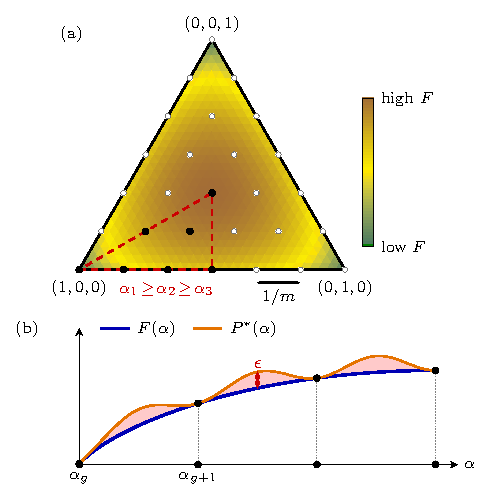
\includegraphics{figures/grid_simplex}
    \caption{Grid discretization of the simplex of spectra for $d_A=3$.
    (a) Different values of $F(\alpha)$ are denoted by different colors. The dots denote the grid $G$, separated by a certain distance $1/m$. Since entanglement measures are symmetric functions on the spectrum, only the points with $\alpha_1\geq\alpha_2\geq\alpha_3$ (dashed region, filled dots) need to be imposed.
    (b) Cut along a one-parameter family of spectra. Although $P^*\leq F$ holds at all grid points, it is possible that $P^*>F$ between any two points by a value $\epsilon$. This value decreases as we refine the grid.}
    \label{fig:grid}
\end{figure}

The proofs of all statements above are given in Appendix~\ref{app:LPconvergence}. We apply this method to estimate the convex roof of the von Neumann entropy of entanglement,
\begin{equation}\label{eq:vonNeumann}
    S(\ket{\psi_{AB}}) = -\tr(\rho_A \log_2 \rho_A),
\end{equation}
where $\rho_A = \tr_B \dyad{\psi_{AB}}$, extended to mixed states via convex roof, which we denote as $E_F=\widehat{S}$. This is known as the entanglement of formation~\cite{Bennett1996EoF}, and it is well known to be difficult to compute~\cite{Chen2005EoF}. To benchmark the method introduced, we use it to estimate $\widehat{S}(\rho_{AB})$ for several families of mixed states $\rho_{AB}$ of different local dimensions, including the main known bound entangled states. The results are given in Fig.~\ref{fig:EoFmain}, and in more detail in Fig.~\ref{fig:EoF} in Appendix~\ref{app:further}.
\detail{Discuss the $E_F$ results state by state: which states and why, why bound entangled states have small $E_F$, how close the lower and upper bounds get (e.g.\ only LB/UB $\approx0.5$ for $3\times3$ bound entangled states at $m=3$, against $\approx0.98$ for $E_1$), the exact two-qubit values as a sanity check, and run times per level. A table of the numbers behind Fig.~\ref{fig:EoFmain} (in the appendix if long) makes them citable.}

% Shared colors and styles of the figures. Every figure reads its data from figures/data/*.csv, written by
% experiments/make_figures.py (comma separated, header row, nan for missing values: pgfplots skips those points).
\definecolor{cA}{HTML}{2a78d6}\definecolor{cB}{HTML}{eb6834}\definecolor{cC}{HTML}{1baf7a}%
\definecolor{cD}{HTML}{4a3aa7}\definecolor{cE}{HTML}{c03b7a}\definecolor{cF}{HTML}{8a6d1f}\definecolor{cGray}{HTML}{8a8984}%
\definecolor{lvA}{HTML}{c6dbf5}\definecolor{lvB}{HTML}{93bbec}\definecolor{lvC}{HTML}{5e98e0}%
\definecolor{lvD}{HTML}{2a78d6}\definecolor{lvE}{HTML}{174a8c}\definecolor{lvF}{HTML}{1baf7a}%
%
% \namedbars{csv file}{ylabel}{title}: lower bounds of the named states at every level, divided by the reference `ref`
% (printed above each state at height `label_y`), with the two upper bounds as markers. Columns: see named_csv in
% make_figures.py. The state positions (`pos`) leave a gap at x = 10 between the PPT and the NPT states.
\providecommand{\namedbar}[3]{% fill, column, offset
  \addplot[ybar, bar width=0.13, bar shift=0pt, draw=none, fill=#1, area legend]
    table[x expr=\thisrow{pos}+#3, y expr=\thisrow{#2}/\thisrow{ref}] {\namedfile};}
\providecommand{\namedbars}[3]{%
  \def\namedfile{#1}%
  \begin{tikzpicture}
    \begin{axis}[width=\textwidth, height=0.29\textwidth, ymin=0, ymax=1.38, xmin=0.3, xmax=14.7,
      ylabel={#2}, ytick={0,0.25,0.5,0.75,1}, xtick=data, xticklabels from table={#1}{state},
      table/col sep=comma, xticklabel style={rotate=35, anchor=north east, font=\scriptsize, inner sep=1pt},
      tick label style={font=\footnotesize}, label style={font=\small}, title={#3}, title style={font=\small,
      yshift=8pt}, clip=false, legend style={font=\scriptsize, at={(0.5,-0.42)}, anchor=north, legend columns=4,
      draw=none, /tikz/every even column/.append style={column sep=6pt}}, legend cell align=left,
      ytick style={draw=none}, xtick style={draw=none}, ymajorgrids, grid style={cGray!25}]
      \addplot[draw=none, forget plot] table[x=pos, y expr=0] {#1};% the ticks (xtick=data)
      \namedbar{lvA}{lb12}{-0.325}\addlegendentry{LB $(1,2)$}
      \namedbar{lvB}{lb13}{-0.195}\addlegendentry{LB $(1,3)$}
      \namedbar{lvC}{lb22}{-0.065}\addlegendentry{LB $(2,2)$}
      \namedbar{lvD}{lb23}{0.065}\addlegendentry{LB $(2,3)$}
      \namedbar{lvE}{lb33}{0.195}\addlegendentry{LB $(3,3)$}
      \namedbar{lvF}{lb24}{0.325}\addlegendentry{LB $(2,4)$}
      \addplot[only marks, mark=diamond*, mark size=2.2pt, cB, mark options={draw=white, line width=0.4pt}]
        table[x expr=\thisrow{pos}-0.14, y expr=\thisrow{ub_extract}/\thisrow{ref}] {#1};
      \addlegendentry{UB: extracted ($k=m=3$)}
      \addplot[only marks, mark=x, mark size=2.4pt, black, thick]
        table[x expr=\thisrow{pos}+0.14, y expr=\thisrow{ub_hjw}/\thisrow{ref}] {#1};
      \addlegendentry{UB: HJW}
      \addplot[only marks, mark=none, nodes near coords={$\pgfplotspointmeta$}, point meta=explicit symbolic,
        nodes near coords style={anchor=south, font=\tiny, inner sep=1pt}, forget plot]
        table[x=pos, y=label_y, meta=ref_label] {#1};
      \draw[cGray] (axis cs:0.3,1) -- (axis cs:14.7,1);
      \draw[cGray, densely dashed] (axis cs:10,0) -- (axis cs:10,1.38);
      \node[font=\scriptsize, anchor=south] at (axis cs:5,1.38) {PPT (bound entangled)};
      \node[font=\scriptsize, anchor=south] at (axis cs:12.5,1.38) {NPT};
    \end{axis}
  \end{tikzpicture}}
%
\begin{figure}[htbp]
  \centering
  \begin{tikzpicture}
    \def\file{figures/data/named_EF_main.csv}
    \begin{axis}[width=0.7\textwidth, height=0.43\textwidth, ymin=0, ymax=1.16, xmin=0.4, xmax=8.6,
      ylabel={$E_{F,\mathrm{LB}}\,/\,\mathrm{UB}$}, ytick={0,0.25,0.5,0.75,1}, xtick=data,
      xticklabels from table={\file}{state}, table/col sep=comma,
      xticklabel style={rotate=35, anchor=north east, font=\scriptsize, inner sep=1pt},
      tick label style={font=\footnotesize}, label style={font=\small}, clip=false,
      ytick style={draw=none}, xtick style={draw=none}, ymajorgrids, grid style={cGray!25}]
      \addplot[ybar, bar width=0.55, bar shift=0pt, draw=none, fill=lvF]
        table[x=pos, y expr=\thisrow{lb_best}/\thisrow{ref}] {\file};
      \addplot[only marks, mark=none, nodes near coords={$\pgfplotspointmeta$}, point meta=explicit symbolic,
        nodes near coords style={anchor=south, font=\tiny, inner sep=1pt}]
        table[x=pos, y expr=1, meta=ref_label] {\file};
      \draw[cGray] (axis cs:0.4,1) -- (axis cs:8.6,1);
      \draw[cGray, densely dashed] (axis cs:6,0) -- (axis cs:6,1.16);
      \node[font=\scriptsize, anchor=south] at (axis cs:3,1.16) {PPT (bound entangled)};
      \node[font=\scriptsize, anchor=south] at (axis cs:7.5,1.16) {NPT};
    \end{axis}
  \end{tikzpicture}
  \caption{Best lower bound on the entanglement of formation $E_F$ for different PPT and NPT states, from the SDP with embedded LP at level $(k,m)=(2,4)$, divided by the best upper bound UB printed above each state. For two qubits, UB is the exact convex roof (marked $^*$). All levels of the hierarchy and both upper bounds, for more states, are shown in Fig.~\ref{fig:EoF}.}
  \label{fig:EoFmain}
\end{figure}


% =====================================================================
\chapter{LOCC convertibility}\label{ch:locc}
Finally, let us demonstrate how the presented approach allows us to determine whether certain pairs of states can be transformed by means of LOCC. To date, and to the best of our knowledge, the only criteria known for this problem are restricted to qubits and very special families of states~\cite{Chitambar2014LOCC,Gour2005InfiniteConditions}.

We can extend the method above to tackle the problem of LOCC convertibility from pure to mixed states, which is in principle an optimization over multiple non-polynomial functions.
According to Ref.~\cite{Jonathan_1999}, a pure state $\ket{\psi}$ can be converted into an ensemble $\{p_i, \ket{\psi_i}\}$ by LOCC if and only if
\begin{equation}\label{eq:JPcriterion}
    E_j(\psi) \geq \sum_i p_i E_j(\psi_i)\qquad \text{for all } j=1,\dots,d_A-1,
\end{equation}
where $E_j$ are the Vidal monotones~\eqref{eq:Vidal}.
Hence, $\ket{\psi}$ can be converted into a mixed state $\rho$ if and only if some decomposition of $\rho$ satisfies all these inequalities simultaneously.
\detail{Explain the Jonathan--Plenio criterion: what converting a pure state into an ensemble means (local operations with flagged outcomes), why it reduces to the Vidal monotones, and why converting into $\rho$ only needs \emph{some} decomposition (the flags are forgotten). A $2\times2$ example where the answer is known lets the reader check the method.}

This is not straightforward to verify, since the decompositions of $\rho$ minimizing each monotone $E_j$ might be different. Assuming we don't use a grid of spectra, let $\mathcal{P}_j$ be the set of polynomials $P_j$ such that $P_j(\a) \leq E_j(\a)$ on all spectra. We want to solve the following optimization problem
\begin{equation}
    \widetilde{s}_k = \max_t\max_{P_j\in\mathcal{P}_j} \min_{\Omega_k} \ \sum_j t_j\Big(\tr\left((O_{P_j}\otimes\I^B)\Omega_k\right)-E_j(\psi)\Big),
\end{equation}
where $t$ is a probability vector. If $\widetilde{s}_k > 0$, then there is at least one Vidal monotone that is not satisfied and LOCC conversion is not possible.

We convert this into an SDP by combining the LPs of Chapter~\ref{sec:LP} for all the $E_j$ into a single SDP and enforcing the polynomial constraints on a grid of spectra.
This gives us the following optimization, where $\mathcal{P}^G_j$ is the set of polynomials satisfying the grid constraint:
\begin{align}\label{eq:LOCCminmaxt}
    s_k=\min_{\Omega_k} \max_t \max_{P_j\in\mathcal{P}^G_j}\ \sum_j t_j\Big(\tr\left((O_{P_j}\otimes\I^B)\Omega_k\right)-E_j(\psi)\Big).
\end{align}
We can swap the $\max$ and $\min$ since the objective is bilinear and the set of $\Omega_k$ is convex and compact (Sion's theorem~\cite{Sion1958}).
\detail{Explain in words why the weights $t_j$ appear: the certificate is a convex combination of the violated inequalities.}
The complete SDP is given in Appendix~\ref{app:LOCC}. From its dual, we can extract the weights $t_j^*$ and polynomials $Q_j^* = t_j^* P_j^*$ that satisfy $Q^*_j\leq t^*_jE_j$ on the grid.

As shown in Chapter~\ref{sec:extractingTheDecomposition}, we can extract the decomposition from the result of the SDP. This leads us to a certificate that certain pure-to-mixed LOCC transformations are possible via Eq.~\eqref{eq:JPcriterion}. This can be summarized as follows.

\begin{result}
By extracting a decomposition $\{p_i, \ket{\psi_i}\}$, we can verify whether it satisfies Eq.~\eqref{eq:JPcriterion} for a certain input state $\ket{\psi}$, and therefore determine whether they can be transformed with LOCC.
\end{result}
However, unlike for the bounds for polynomial and non-polynomial measures, it may not always be possible to extract the correct decomposition. This comes from the fact that there may not exist a decomposition of $\rho$ into linearly independent terms that satisfies the criterion of Eq.~\eqref{eq:JPcriterion}, which makes it very difficult for the algorithms of Chapter~\ref{sec:extractingTheDecomposition} to find the underlying decomposition.
Instead, a similar strategy allows us to obtain a complete no-go criterion to discard entanglement transformations.

\begin{result}\label{thm:LOCC}
We obtain a complete hierarchy for LOCC non-convertibility in the following sense:
    \begin{enumerate}
    \item Let $\epsilon_j=\max_{\a}\left(Q^*_j(\a)-t^*_jE_j(\a)\right)$, taken over all spectra, be the grid errors of the polynomials returned by the solver.
    If $s_k>\sum_j\epsilon_j$ for some $k$, then $\ket{\psi}$ cannot be converted into $\rho$ by LOCC.
    \item In the limit where the grid $G$ is continuous and covers all possible spectra $\alpha$, for any $\ket{\psi}$ and $\rho$, if $\ket{\psi} \overset{\text{LOCC}}{\nrightarrow} \rho$, there is a finite level $k$ at which $\widetilde{s}_k > 0$.
    \end{enumerate}
\end{result}
The proof is given in Appendix~\ref{app:LOCCchap}. Notice that although the grid will always be discrete in practical computations, by continuity the second item suggests that finer grids lead to tighter criteria. Numerically, we verify that this is the case for all states tested.
\detail{Describe Fig.~\ref{fig:locc} in detail: the states and parameters, the region certified non-convertible, where extraction certified convertibility, and where neither test decides. Report how often the extraction succeeds, since the convertibility test is heuristic.}

% Shared colors and styles of the figures. Every figure reads its data from figures/data/*.csv, written by
% experiments/make_figures.py (comma separated, header row, nan for missing values: pgfplots skips those points).
\definecolor{cA}{HTML}{2a78d6}\definecolor{cB}{HTML}{eb6834}\definecolor{cC}{HTML}{1baf7a}%
\definecolor{cD}{HTML}{4a3aa7}\definecolor{cE}{HTML}{c03b7a}\definecolor{cF}{HTML}{8a6d1f}\definecolor{cGray}{HTML}{8a8984}%
\definecolor{lvA}{HTML}{c6dbf5}\definecolor{lvB}{HTML}{93bbec}\definecolor{lvC}{HTML}{5e98e0}%
\definecolor{lvD}{HTML}{2a78d6}\definecolor{lvE}{HTML}{174a8c}\definecolor{lvF}{HTML}{1baf7a}%
%
% \namedbars{csv file}{ylabel}{title}: lower bounds of the named states at every level, divided by the reference `ref`
% (printed above each state at height `label_y`), with the two upper bounds as markers. Columns: see named_csv in
% make_figures.py. The state positions (`pos`) leave a gap at x = 10 between the PPT and the NPT states.
\providecommand{\namedbar}[3]{% fill, column, offset
  \addplot[ybar, bar width=0.13, bar shift=0pt, draw=none, fill=#1, area legend]
    table[x expr=\thisrow{pos}+#3, y expr=\thisrow{#2}/\thisrow{ref}] {\namedfile};}
\providecommand{\namedbars}[3]{%
  \def\namedfile{#1}%
  \begin{tikzpicture}
    \begin{axis}[width=\textwidth, height=0.29\textwidth, ymin=0, ymax=1.38, xmin=0.3, xmax=14.7,
      ylabel={#2}, ytick={0,0.25,0.5,0.75,1}, xtick=data, xticklabels from table={#1}{state},
      table/col sep=comma, xticklabel style={rotate=35, anchor=north east, font=\scriptsize, inner sep=1pt},
      tick label style={font=\footnotesize}, label style={font=\small}, title={#3}, title style={font=\small,
      yshift=8pt}, clip=false, legend style={font=\scriptsize, at={(0.5,-0.42)}, anchor=north, legend columns=4,
      draw=none, /tikz/every even column/.append style={column sep=6pt}}, legend cell align=left,
      ytick style={draw=none}, xtick style={draw=none}, ymajorgrids, grid style={cGray!25}]
      \addplot[draw=none, forget plot] table[x=pos, y expr=0] {#1};% the ticks (xtick=data)
      \namedbar{lvA}{lb12}{-0.325}\addlegendentry{LB $(1,2)$}
      \namedbar{lvB}{lb13}{-0.195}\addlegendentry{LB $(1,3)$}
      \namedbar{lvC}{lb22}{-0.065}\addlegendentry{LB $(2,2)$}
      \namedbar{lvD}{lb23}{0.065}\addlegendentry{LB $(2,3)$}
      \namedbar{lvE}{lb33}{0.195}\addlegendentry{LB $(3,3)$}
      \namedbar{lvF}{lb24}{0.325}\addlegendentry{LB $(2,4)$}
      \addplot[only marks, mark=diamond*, mark size=2.2pt, cB, mark options={draw=white, line width=0.4pt}]
        table[x expr=\thisrow{pos}-0.14, y expr=\thisrow{ub_extract}/\thisrow{ref}] {#1};
      \addlegendentry{UB: extracted ($k=m=3$)}
      \addplot[only marks, mark=x, mark size=2.4pt, black, thick]
        table[x expr=\thisrow{pos}+0.14, y expr=\thisrow{ub_hjw}/\thisrow{ref}] {#1};
      \addlegendentry{UB: HJW}
      \addplot[only marks, mark=none, nodes near coords={$\pgfplotspointmeta$}, point meta=explicit symbolic,
        nodes near coords style={anchor=south, font=\tiny, inner sep=1pt}, forget plot]
        table[x=pos, y=label_y, meta=ref_label] {#1};
      \draw[cGray] (axis cs:0.3,1) -- (axis cs:14.7,1);
      \draw[cGray, densely dashed] (axis cs:10,0) -- (axis cs:10,1.38);
      \node[font=\scriptsize, anchor=south] at (axis cs:5,1.38) {PPT (bound entangled)};
      \node[font=\scriptsize, anchor=south] at (axis cs:12.5,1.38) {NPT};
    \end{axis}
  \end{tikzpicture}}
%
% Classes (column `class` of locc.csv): 0 psi->rho certified (Theorem LOCC (ii)), 1 psi->rho excluded (Theorem LOCC (i)),
% 2 inconclusive, 3 incomparable (only if SHOW_REVERSE in make_figures.py). 31 x 31 grid, rows ordered by p then theta.
\begin{figure}[tbp]
  \centering
  \begin{tikzpicture}
    \begin{axis}[width=0.55\textwidth, height=0.48\textwidth, xlabel={$\theta/\pi$}, ylabel={$p$},
      xtick={0,0.05,0.1,0.15,0.2,0.25}, xticklabel style={/pgf/number format/fixed, /pgf/number format/precision=2},
      xmin=-0.00416668, xmax=0.254167,
      ymin=-0.0166665, ymax=1.01667, axis on top,
      colormap={locc}{color(0)=(cA!55) color(1)=(cB!60) color(2)=(cGray!45) color(3)=(cC!60)},
      colormap access=direct,
      tick label style={font=\footnotesize}, label style={font=\small}, name=ax]
      \addplot[matrix plot*, mesh/cols=31, point meta=explicit, forget plot]
        table[col sep=comma, x=theta_over_pi, y=p, meta=class] {figures/data/locc.csv};
    \end{axis}
    \node[anchor=south, font=\scriptsize, inner sep=1pt] at ([yshift=3pt]ax.north) {%
      \begin{tabular}{@{}l@{\hspace{1.2em}}l@{}}
      \tikz\fill[cA!55] (0,0) rectangle (2mm,2mm); $\psi\to\rho$ (decomposition) &
      \tikz\fill[cB!60] (0,0) rectangle (2mm,2mm); $\psi\nrightarrow\rho$ (SDP) \\
      \tikz\fill[cGray!45] (0,0) rectangle (2mm,2mm); inconclusive
      \end{tabular}};
  \end{tikzpicture}
  \caption{LOCC convertibility from the pure state $\ket{\psi}$ with entanglement spectrum
  $(0.6,0.3,0.1)$ to the two-qutrit states
  $\rho(p,\theta)=p\dyad{\Phi_3}+(1-p)\dyad{\chi_\theta}$, with $\ket{\Phi_3}$ maximally entangled and
  $\ket{\chi_\theta}=\cos\theta\ket{00}+\sin\theta\ket{11}$, from the SDP of Eq.~\eqref{eq:LOCCminmaxt} at level $(k,m)=(3,4)$.}
  \label{fig:locc}
\end{figure}


% =====================================================================
\chapter{Libraries}\label{ch:libraries}
\section{\texttt{schur-weyl}}
When implementing the method, we found very few online resources providing the tools from Schur--Weyl duality that we needed for our code. At the start of the project we used SageMath~\cite{sagemath}, which provides the character tables needed to build the isotypic projectors of Eq.~\eqref{eq:isotypic}, which are hard to compute in general, as well as Schur polynomials. However, SageMath is heavy (about 3\,GB) and still required a lot of code to build the tools we needed.
We therefore built a small Python package, \href{https://github.com/AVlyx/schur-weyl}{\texttt{schur-weyl}}~\cite{schurWeyl}, that provides the tools used in this project.

The content of the package is listed in Table~\ref{tab:schurweyl}.
\begin{table}[h]
\centering\small\renewcommand{\arraystretch}{1.15}
\begin{tabular}{@{}lp{11.2cm}@{}}
\hline
Module & Contents \\
\hline
\texttt{young\_diagrams} & Partitions and the relevant helpers \\
\texttt{dimensions} & $f^\lambda=\dim\mathcal S^\lambda_k$ and $\dim\mathcal U^\lambda_d$ \\
\texttt{tableaux} & Standard and semi-standard Young tableaux, Kostka numbers\\
\texttt{symmetric\_group} & Permutations, composition of permutations, inverse, cycle type of a permutation, conjugacy class sizes \\
\texttt{character} & Characters $\chi^\lambda$ of $S_k$ \\
\texttt{symmetric\_functions} & Schur polynomials, power sums, monomial symmetric polynomials and their expansion in the Schur basis \\
\texttt{isotypic} & Isotypic projectors $\Pi^\lambda$ \\
\texttt{sw\_measure} & Weak Schur sampling distribution $f^\lambda s_\lambda(\spec\rho)$ \\
\texttt{schur\_transform} & Schur transform: a real orthogonal matrix block-diagonalising the actions of $S_k$ and $GL_d$ simultaneously \\
\hline
\end{tabular}
\caption{Modules of \texttt{schur-weyl}~\cite{schurWeyl}.}
\label{tab:schurweyl}
\end{table}

\section{\texttt{bound-entangled}}
As the project started, our first goal was to test the hierarchy above to measure the Schmidt number and see whether it is possible to do better than projecting on the antisymmetric projector. This is not possible by Lemma~\ref{lem:lifting}.

To test this, we needed access to families of states on which we could run the SDP. At the time, the SDP was very costly, at about 15\,GB of memory at level $k=3$ for two-qutrit states, which led us to mostly test it on the separability problem for bound entangled states, since PPT entangled states are not detected by the PPT criterion.
This led us to build a \href{https://github.com/AVlyx/bound-entangled}{repository} of families of bound entangled states, \texttt{bound-entangled}~\cite{boundEntangled}.

The states it contains are listed in Table~\ref{tab:boundentangled}.
\begin{table}[h]
\centering\small\renewcommand{\arraystretch}{1.15}
\begin{tabular}{@{}lp{12.3cm}@{}}
\hline
Space & States \\
\hline
$\C^2\otimes\C^4$ & Horodecki $2\times4$ state \\
$\C^3\otimes\C^3$ & Horodecki $3\times3$ state, chessboard states, cross-hatch grid state, Vértesi--Brunner state violating a Bell inequality, steerable state disproving the stronger Peres conjecture, Tiles and Pyramid UPB states, six-parameter family of UPBs generalising them \\
$\C^4\otimes\C^4$ & Piani state \\
$\C^5\otimes\C^5$ & Grid state with Schmidt number 3\\
$\C^d\otimes\C^d$ & Yu--Oh states, GenTiles1 UPB states, private-singlet states of Badzi\k{a}g et al., second family of PPT singlets, Horodecki state generalised to $\C^2\otimes\C^d$, Breuer states \\
$\C^m\otimes\C^n$ & Grid states and their generalisation to hypergraphs, GenTiles2 UPB states \\
Multipartite & Smolin state, generalised Smolin states, quasi-DS states \\
\hline
\end{tabular}
\caption{States implemented in \texttt{bound-entangled}~\cite{boundEntangled}, by Hilbert space. UPB: unextendible product basis.}
\label{tab:boundentangled}
\end{table}

% =====================================================================
\chapter{Conclusions}\label{ch:conclusions}

By using a unitarily invariant basis of projectors, which lets us compute polynomials of the entanglement spectrum on pure states, we have introduced an SDP formulation to bound any entanglement measure of bipartite mixed states. This method was extended to the problem of LOCC convertibility with a hierarchy of certificates of non-convertibility and a heuristic approach towards certifying convertibility.
A natural direction for future work would be to see how this method can be extended to the multipartite setting. I would also like to see how we could further optimize the SDP, either by increasing the convergence rate by adding more separability constraints along the systems of $\Omega_k$ such as realignment criterion constraints, or by improving the symmetry reductions and the choice of grid points for the LP.


\bigskip
{\em Contributions.} This report is based on the paper~\cite{ourPaper}, written with Albert Rico and Otfried G\"uhne, and a significant part of the text is adapted from it. I wrote the main body of the paper as well as the appendices with some edits from my supervisors. The conclusion and introduction of the paper were mainly written by my co-authors. I also developed the software libraries.

{\em AI statement.} The ideas, methodology, proof strategies and the project scope were designed by the authors. I used AI coding tools (Claude Opus 4.8--5.5) to write and debug part of the code, including the software libraries, to run and plot numerical experiments and to check proof calculations. All results were validated by me.

{\em Acknowledgements.} Thank you to Albert Rico and Otfried G\"uhne for welcoming me into the group and for all their help during the internship. Thank you to everyone from the University of Siegen for the great time I had.
% =====================================================================
\appendix

\chapter{Representation theory and lifting}\label{app:repTheory}
\deeper{Derive the isotypic projector of Eq.~\eqref{eq:isotypic} from the orthogonality of characters (it is the central idempotent of the group algebra) and show that the $\Pi^\lambda$ are orthogonal projectors summing to the identity. Commutation with $g^{\otimes k}$ follows from Eq.~\eqref{eq:PerUniCommute} in one line; write it.}
\deeper{Prove the weak Schur sampling formula $\tr(\Pi^\lambda\rho_A^{\otimes k})=f^\lambda s_\lambda(\spec\rho_A)$: by unitary invariance take $\rho_A$ diagonal; on $\mathcal S^\lambda_k\otimes\mathcal U^\lambda_d$ the operator $\rho_A^{\otimes k}$ acts as $\I_{f^\lambda}\otimes q_\lambda(\rho_A)$, and the character of the $GL_d$ irrep at a diagonal matrix is the Schur polynomial. Check it by hand at $k=2$: $\tr(\Pi^{(2)}\rho^{\otimes2})=(1+\tr\rho^2)/2=s_{(2)}$.}

\section{Lifting to higher degree}\label{sec:lifting}
\begin{lemma}\label{lem:lifting}
    Let $P$ be a homogeneous symmetric polynomial of degree $m$ with $m < k$. Let $P_k$ be its lift to degree $k$ such that $P_k(\a) = P(\a) \left(\sum_i \a_i \right)^{k-m} = P(\a)$ where $\a$ is the spectrum of a state $\rho_A$.
    Then, for every $\Omega_k$ acting on $(\C^{d_A} \otimes \C^{d_B})^{\otimes k}$, which is permutation invariant across all $k$ copies of $\C^{d_A} \otimes \C^{d_B}$,
    \begin{equation}
        \tr(O_P^{A_1,\dots, A_m} \otimes \I^{A_{m+1}, \dots, A_k} \otimes \I^{B} \Omega_k) = \tr(O_{P_k}^A \otimes \I^B \Omega_k).
    \end{equation}
\end{lemma}
\begin{proof}
    Let $\mathcal{T} = \frac{1}{k!}\sum_{\pi \in S_k} \pi \ O_P \otimes \I^{\otimes (k-m)} \ \pi^\dagger$ be the twirl of $O_P \otimes \I^{\otimes (k-m)}$ over $S_k$. Obviously $\mathcal{T}$ commutes with every permutation in $S_k$, and, since it is a linear combination of permutations, we can write it as a sum of isotypic projectors $\mathcal{T} = \sum_{\lambda \vdash k} a_\lambda \Pi^\lambda$ for some coefficients $a_\lambda$.

    For any $\rho_A$ with spectrum $\a$, since $\rho_A^{\otimes k}$ is permutation invariant,
    \begin{equation}
        \tr(\mathcal{T}\rho_A^{\otimes k}) = \tr\Big(\frac{1}{k!} \sum_{\pi \in S_k} \pi\, O_P \otimes \I\, \pi^\dagger \rho_A^{\otimes k}\Big)= \tr(O_P \otimes \I\, \rho_A^{\otimes k}).
    \end{equation}
    Thus $\mathcal{T}$ and $O_{P_k}$ have the same expectation value $P_k(\a)$ on every $\rho_A^{\otimes k}$, and since both are combinations of isotypic projectors and the Schur polynomials are linearly independent, $\mathcal{T} = O_{P_k}$.
    Finally,
    \begin{align}
        &\tr(O_P^{A_1,\dots, A_m} \otimes \I^{A_{m+1}, \dots, A_k} \otimes \I^{B} \Omega_k)\\
        =& \tr\Big( \frac{1}{k!}\sum_{\pi \in S_k} O_P^{A_1,\dots, A_m} \otimes \I^{A_{m+1}, \dots, A_k} \otimes \I^{B} \pi^\dagger \Omega_k \pi\Big)\\
        =& \tr\Big( \frac{1}{k!}\sum_{\pi \in S_k}  \pi O_P^{A_1,\dots, A_m} \otimes \I^{A_{m+1}, \dots, A_k} \otimes \I^{B} \pi^\dagger \Omega_k\Big)\\
        =& \tr( O_{P_k} \otimes \I^{B} \Omega_k).
    \end{align}
\end{proof}
\deeper{Two steps deserve a sentence each: why $O_P\otimes\I^{\otimes(k-m)}$ is a linear combination of permutations of $S_k$ (embed $S_m\subset S_k$), and why a permutation-invariant element of the span of permutations is a combination of the $\Pi^\lambda$ (the centre of the group algebra is spanned by the class sums, equivalently by the central idempotents). Also note that both $s_\lambda$ and $\Pi^\lambda_A$ vanish for $\ell(\lambda)>d_A$, so linear independence is only needed for $\ell(\lambda)\le d_A$.}

% =====================================================================
\chapter{Proofs for the SDP hierarchy}\label{app:proofsHierarchy}

\section{Convergence}\label{app:ProofCongNonExtHier}
\begin{proof}[Proof of Result~\ref{thm:ConvergenceSDPcroof}]
We consider a polynomial $P$ of degree $m$. At level $k \geq m$ of the hierarchy, we obtain the optimal solution $\Omega_k$, with $P_{{\rm LB}_k}(\rho) = \tr(O_P\, \Omega_m)$ where $\Omega_m = \tr_{m+1,\dots, k}(\Omega_k)$ is the $m$-copy marginal of $\Omega_k$.
By the de Finetti theorem for Bose-symmetric states~\cite[Thm.~II.8]{Christandl_2007}, for every feasible $\Omega_k$, there is an $\omega_m = \int \dyad{\phi}^{\otimes m} d\mu(\phi)$ such that
\begin{equation}
    \left\|\Omega_m - \omega_m\right\|_1 \leq \epsilon
\end{equation}
with $\epsilon = \tfrac{4 D m}{k}$. By Carath\'eodory's theorem, since the space is finite-dimensional, we can write $\omega_m = \sum_i p_i \dyad{\phi_i}^{\otimes m}$. Here, $\omega_m$ is associated to a decomposition $\{p_i, \ket{\phi_i}\}_i$ corresponding to a state $\sigma$ and $\tr(O_P \,\omega_m) \geq \widehat{P}(\sigma)$. Since the partial trace is contractive, $\left\|\rho - \sigma\right\|_1 = \left\|\tr_{2,\dots, m}(\Omega_m - \omega_m)\right\|_1 \leq \epsilon$.

Then, by H\"{o}lder inequality \eqref{eq:HolderStep}, by definition of the convex roof \eqref{eq:croofstep} and from the continuity of the convex roof of a continuous function in finite dimensions \eqref{eq:contConv}~\cite[Thm.~6.1]{Bucicovschi2013},
\begin{align}
    \tr(O_P \Omega_m) &\geq \tr(O_P\omega_m) - \epsilon\|O_P\|_\infty \label{eq:HolderStep}\\
    &\geq \widehat{P}(\sigma) - \epsilon\|O_P\|_\infty \label{eq:croofstep}\\
    &\geq \widehat{P}(\rho) - \delta(\epsilon) - \epsilon\|O_P\|_\infty \label{eq:contConv}
\end{align}
with $\delta(\epsilon) \to 0$.

Hence, $\widehat{P}{(\rho)} \geq P_{{\rm LB}_k}(\rho) \geq \widehat{P}{(\rho)} -\delta(\epsilon) - \epsilon\|O_P\|_\infty$, and therefore $P_{{\rm LB}_k}(\rho) \to \widehat{P}(\rho)$ as $k \to \infty$.
\end{proof}
\deeper{This is the main theorem; expand the proof. State the de Finetti theorem precisely (hypotheses, norm, constant) and check $\epsilon=4Dm/k$ against Ref.~\cite{Christandl_2007}, with $D=d_Ad_B$ as the single-copy dimension and $\Omega_k$ normalised by the marginal constraint. Explain why Carath\'eodory turns the integral into a finite sum. State the continuity theorem of Ref.~\cite{Bucicovschi2013} that you use. Bound $\|O_P\|_\infty\le\max_\lambda|c_\lambda|/f^\lambda$ (the $\Pi^\lambda$ are orthogonal). If possible, give an explicit rate in $k$ for one measure, e.g.\ the linear entropy, using an explicit continuity bound for its convex roof.}

\section{Monotonicity in the level}\label{app:monotonicity}
In the full SDP, at level $k+1$, we obtain the optimal solution $\Omega_{k+1}$. Let $O_k$ be the observable at level $k$ and $O_{k+1}$ be its lift to level $k+1$. Then, $P_{{\rm LB}_{k+1}} = \tr(O_{k+1} \Omega_{k+1})=\tr(O_k \otimes \I \ \Omega_{k+1})$ according to Lemma~\ref{lem:lifting}. At level $k$, $\tr_{A_{k+1}B_{k+1}}(\Omega_{k+1})$ is also in the feasible set -- PPT across copies, permutation invariant, first marginal equal to $\rho$ and PSD -- with $\tr(O_k \tr_{A_{k+1}B_{k+1}}(\Omega_{k+1})) = P_{{\rm LB}_{k+1}}$. Then, $P_{{\rm LB}_{k+1}} \geq P_{{\rm LB}_{k}}$.
We can use the same argument in $k$ and $m$ for the simplified SDP.
\deeper{Write out the simplified case instead of ``the same argument'': which registers are traced out to go from $(k,m+1)$ to $(k,m)$ and from $(k+1,m)$ to $(k,m)$, and which constraints survive each step.}

\section{Simplified relaxation}\label{sec:pptReps}
Since $\Phi_{k,m}$ can be assumed invariant under permutations of $A_1B_1, \dots, A_kB_k$ and $A_{k+1}, \dots, A_m$, it suffices to impose partial transpose conditions on the tuples $(i, j)$ where each tuple means taking the partial transpose on the first $i$ full-copy registers and the first $j$ marginal registers. One such set of representatives is $\{(i,j):0\leq i\leq k,\ 0\leq j<\tfrac{m-k}{2}\}\ \cup\ \{(i,\tfrac{m-k}{2}):0\leq i\leq\lfloor k/2\rfloor\}$ where the second set is only present for even $m-k$ and the tuple $(0,0)$ is excluded. By permutation invariance, adding any other PPT constraint would be redundant and not increase the bound. We also tried other sets of PPT constraints, such as enforcing them on $\tr_{B_1 \dots B_k}(\Phi_{k,m})$, which would have reduced the number of PPT constraints and their cost since they act on a smaller matrix, but the bounds we got were much worse.
\detail{Check each constraint on $\omega_{k,m}$ as for the full SDP, and give the counting argument behind the set of PPT representatives, with a small case such as $k=2$, $m=4$.}
\deeper{Write out $P_{{\rm LB}_k}\le P_{{\rm LB}_{k,m}}$. It needs the lifting lemma on the $A$ registers only, using that $\tr_B\Phi_{k,m}$ is permutation invariant (the fourth constraint), to move $O_P$ from $A_1,\dots,A_m$ to $A_1,\dots,A_k$; otherwise the objective is not defined on $\Phi_k$.}

% =====================================================================
\chapter{Symmetry reductions and memory}\label{app:SymRed}
Throughout this appendix, a single copy of $\C^{d_A}\otimes\C^{d_B}$ is identified with $\C^D$, with orthonormal basis $\{\ket{j}\}_{j=0}^{D-1}$.

\section{Restriction to the symmetric subspace}
The symmetric subspace $\text{Sym}^k(\C^D)$ has an orthonormal basis indexed by occupation vectors. The occupation vector denoted $\nu(i_1,\dots,i_k)\in\N^D$ of a basis vector $\ket{i_1,\dots,i_k}\in(\C^D)^{\otimes k}$ has entries $\nu_j$ equal to the number of times $j$ appears in $(i_1,\dots,i_k)$. For example, $\nu(0,1,2,0,0,1,2,2)=(3,2,3)$ for $D=3$, $k=8$. We define the isometry $V_k:(\C^D)^{\otimes k}\to\text{Sym}^k(\C^D)$ as
\begin{equation}
    V_k = \sum_{i_1, \dots, i_k=0}^{D-1} \binom{k}{\nu(i_1, \dots, i_k)}^{-1/2}\ket{\nu(i_1, \dots, i_k)}\bra{i_1, \dots, i_k},
\end{equation}
where $\binom{k}{\nu}=k!/\prod_j\nu_j!$ is the multinomial coefficient, i.e., the number of basis vectors with occupation vector $\nu$. It has real entries and satisfies $V_kV_k^\dagger=\I_{\text{Sym}^k}$ and $V_k^\dagger V_k=\Pi_{\rm sym}^{k}$. Since every feasible $\Omega_k$ is supported on the symmetric subspace, $\Omega_k=V_k^\dagger\Omega_k^{\rm sym}V_k$ with $\Omega_k^{\rm sym}=V_k\Omega_kV_k^\dagger$, a matrix of size $\binom{k+D-1}{k}$. The objective becomes $\tr\left(V_k(O_P\otimes\I^B)V_k^\dagger\,\Omega_k^{\rm sym}\right)$.
\detail{Add a small worked example of the occupation basis ($D=2$, $k=2$: the three states $\ket{2,0},\ket{1,1},\ket{0,2}$ and $V_2$ as a $3\times4$ matrix).}

\section{First marginal constraint}
Here we wish to encode the condition $\tr_{A_2B_2\dots A_kB_k}(\Omega_k) = \rho$.
We define the occupation vector $\nu_\downarrow$ such that $\ket{\nu_\downarrow} \in \text{Sym}^{k-1}(\C^D)$, and $\ket{\nu_\downarrow + e_j} \in \text{Sym}^k(\C^D)$ has one more element $\ket{j}$, i.e., $(\nu_\downarrow + e_j)_j=(\nu_\downarrow)_j + 1$. Grouping the $\binom{k-1}{\nu_\downarrow}$ tuples $(i_2,\dots,i_k)$ with the same occupation vector and using $\binom{k}{\nu_\downarrow+e_j}=\binom{k-1}{\nu_\downarrow}\frac{k}{\nu_{\downarrow,j}+1}$, we get
\begin{equation}
    \left(\tr_{2,\dots,k}\Omega_k\right)_{jj'}
    =\sum_{\nu_\downarrow}\binom{k-1}{\nu_\downarrow}\frac{\bra{\nu_\downarrow+e_j}\Omega_k^{\rm sym}\ket{\nu_\downarrow+e_{j'}}}{\sqrt{\binom{k}{\nu_\downarrow+e_j}\binom{k}{\nu_\downarrow+e_{j'}}}}
    =\frac1k\tr\!\left(\hat a_{j'}^\dagger\hat a_j\,\Omega_k^{\rm sym}\right),
\end{equation}
with the bosonic creation operators $\hat a_j^\dagger:\text{Sym}^{k-1}(\C^D)\to\text{Sym}^k(\C^D)$,
\begin{equation}
    \hat a_j^\dagger=\sum_{\nu_\downarrow}\sqrt{\nu_{\downarrow,j}+1}\,\ket{\nu_\downarrow+e_j}\bra{\nu_\downarrow}.
\end{equation}
Thus, the marginal constraint becomes the linear constraint $\frac1k\sum_{j,j'}\tr\left(\hat a_{j'}^\dagger\hat a_j\,\Omega_k^{\rm sym}\right)\ket{j}\bra{j'}=\rho$.

\section{Partial-transpose constraints}
Thanks to the permutation symmetry, the partial transpose only depends on the size of the set of transposed copies, and since $\Omega_k^{T_{S^c}}=(\Omega_k^{T_S})^T$, a set and its complement give equivalent constraints. We therefore impose the PPT constraints on the first $l$ copies for $l \in \{1, \dots, \lfloor \tfrac{k}{2} \rfloor\}$. We define the isometry
\begin{equation}
    W_l=(V_l\otimes V_{k-l})V_k^\dagger:\ \text{Sym}^k(\C^D)\to\text{Sym}^l(\C^D)\otimes\text{Sym}^{k-l}(\C^D),
\end{equation}
so that $\Omega_k=(V_l\otimes V_{k-l})^\dagger\,W_l\Omega_k^{\rm sym}W_l^\dagger\,(V_l\otimes V_{k-l})$. Writing $T_l$ also for the transpose of the factor $\text{Sym}^l(\C^D)$ in the occupation basis, the partial transpose becomes
\begin{align}
    \Omega_k^{T_l} &= \left((V_l\otimes V_{k-l})^\dagger\,W_l\Omega_k^{\rm sym}W_l^\dagger\,(V_l\otimes V_{k-l})\right)^{T_l}\\
    &=\left(V_l^T\otimes V_{k-l}^\dagger\right)\,\left(W_l\Omega_k^{\rm sym}W_l^\dagger\right)^{T_l}\,\left(V_l^*\otimes V_{k-l}\right)\\
    &= (V_l\otimes V_{k-l})^\dagger\,\left(W_l\Omega_k^{\rm sym}W_l^\dagger\right)^{T_l}\,(V_l\otimes V_{k-l}),
\end{align}
since $V_l$ is real, so that $V_l^T=V_l^\dagger$ and $V_l^*=V_l$. Conjugating back with $V_l\otimes V_{k-l}$, the condition becomes
\begin{equation}
    \Omega_k^{T_l}\succeq0\iff\left(W_l\,\Omega_k^{\rm sym}W_l^\dagger\right)^{T_l}\succeq0,\qquad 1\leq l\leq\lfloor k/2\rfloor.
\end{equation}
This is the most expensive constraint of the SDP, since it encodes the state in the larger space $\text{Sym}^l(\C^D)\otimes\text{Sym}^{k-l}(\C^D)$ to support the partial transpose. While these constraints are not necessary for the hierarchy to be complete, they help convergence at finite $k$, as shown in Ref.~\cite{Navascues2009}.
\detail{Quantify what the PPT constraints cost and gain: bounds with and without them at the same level, and the size of the $\mathrm{Sym}^l\otimes\mathrm{Sym}^{k-l}$ blocks.}

\section{Real variables}
If $\rho$ is real, the SDP can be restricted to real symmetric matrices. If $\Omega_k$ is feasible, so is its entrywise complex conjugate $\Omega_k^*$, since conjugation commutes with partial traces, partial transposes and the real projector $\Pi_{\rm sym}^k$, and $\rho^*=\rho$. Since the isotypic projectors are linear combinations of permutation matrices with real characters, $O_P$ is real, and
\begin{equation}
    \tr\left((O_P^A \otimes \I^B)\, \Omega_k\right) = \tr\left((O_P^A \otimes \I^B)\, \Omega_k^*\right) = \tr\Big((O_P^A \otimes \I^B)\, \tfrac{\Omega_k + \Omega_k^*}{2}\Big).
\end{equation}
By convexity, $\frac12(\Omega_k+\Omega_k^*)$ is feasible, real and has the same objective value, so the optimum is attained by a real matrix. For the true $\omega_k$, this real matrix is $\frac{1}{2}\sum_i p_i \left(\dyad{\psi_i}^{\otimes k} + \dyad{\psi_i^*}^{\otimes k}\right)$, which corresponds to the decomposition $\{\frac{p_i}{2},\ket{\psi_i}\}\cup\{\frac{p_i}{2},\ket{\psi_i^*}\}$ of $\rho$. The same argument applies to $\Phi_{k,m}$ in the simplified relaxation.
\detail{Add the remark that a real $\rho$ does not imply a real optimal decomposition: the argument only shows that the optimal $\Omega_k$ can be taken real, which corresponds to the symmetrised ensemble with $\ket{\psi_i}$ and $\ket{\psi_i^*}$. Quantify the saving in memory and time on one example.}

\section{Projection onto the support of $\rho$}\label{app:supportReduction}
Let $r = \operatorname{rank} \rho$, and let $V_\rho: \C^D \to \C^r$ be the isometry onto the support of $\rho$, given by the eigenvectors of $\rho$ with nonzero eigenvalue, so that $V_\rho V_\rho^\dagger=\I_r$ and $V_\rho^\dagger V_\rho=\Pi_\rho$, the projector onto the support of $\rho$. Every feasible $\Omega_k$ is supported on $(\operatorname{supp}\rho)^{\otimes k}$: since
\begin{equation}
    \tr\left(((\I-\Pi_\rho)\otimes\I)\,\Omega_k\right)=\tr\left((\I-\Pi_\rho)\rho\right)=0
\end{equation}
and $\Omega_k\succeq0$, we have $((\I-\Pi_\rho)\otimes\I)\,\Omega_k=0$, and by permutation symmetry the same holds on every copy. Hence $\Omega_k=\Pi_\rho^{\otimes k}\Omega_k\Pi_\rho^{\otimes k}$, and
\begin{equation}
    \tr\left((O_P^A\otimes\I^B)\,\Omega_k\right)=\tr\Big(\left(V_\rho^{\otimes k}(O_P^A\otimes\I^B)V_\rho^{\dagger\otimes k}\right)\left(V_\rho^{\otimes k}\Omega_kV_\rho^{\dagger\otimes k}\right)\Big).
\end{equation}
We can therefore equivalently optimize over $\Omega_k^\rho=V_\rho^{\otimes k}\Omega_kV_\rho^{\dagger\otimes k}$ on $(\C^r)^{\otimes k}$ with marginal $V_\rho\rho V_\rho^\dagger$. Bose symmetry is preserved, since $V_\rho^{\otimes k}$ commutes with permutations, and the partial-transpose constraints are equivalent, since $(\Omega_k^\rho)^{T_l}$ and $\Omega_k^{T_l}$ are related in both directions by congruences with $V_\rho$ and $V_\rho^*$. Combined with the symmetric subspace, the variable has size $\binom{k+r-1}{k}$. If $\rho$ is real, $V_\rho$ can be chosen real and the real-variable reduction still applies.

The same argument applies to the simplified relaxation: by the permutation invariance of $\tr_B\Phi_{k,m}$, every $A$ register has reduced state $\rho_A=\tr_B(\rho)$, and therefore all $A$ registers can be encoded on the support of $\rho_A$.

\section{Memory cost}\label{sec:memory}
% Shared colors and styles of the figures. Every figure reads its data from figures/data/*.csv, written by
% experiments/make_figures.py (comma separated, header row, nan for missing values: pgfplots skips those points).
\definecolor{cA}{HTML}{2a78d6}\definecolor{cB}{HTML}{eb6834}\definecolor{cC}{HTML}{1baf7a}%
\definecolor{cD}{HTML}{4a3aa7}\definecolor{cE}{HTML}{c03b7a}\definecolor{cF}{HTML}{8a6d1f}\definecolor{cGray}{HTML}{8a8984}%
\definecolor{lvA}{HTML}{c6dbf5}\definecolor{lvB}{HTML}{93bbec}\definecolor{lvC}{HTML}{5e98e0}%
\definecolor{lvD}{HTML}{2a78d6}\definecolor{lvE}{HTML}{174a8c}\definecolor{lvF}{HTML}{1baf7a}%
%
% \namedbars{csv file}{ylabel}{title}: lower bounds of the named states at every level, divided by the reference `ref`
% (printed above each state at height `label_y`), with the two upper bounds as markers. Columns: see named_csv in
% make_figures.py. The state positions (`pos`) leave a gap at x = 10 between the PPT and the NPT states.
\providecommand{\namedbar}[3]{% fill, column, offset
  \addplot[ybar, bar width=0.13, bar shift=0pt, draw=none, fill=#1, area legend]
    table[x expr=\thisrow{pos}+#3, y expr=\thisrow{#2}/\thisrow{ref}] {\namedfile};}
\providecommand{\namedbars}[3]{%
  \def\namedfile{#1}%
  \begin{tikzpicture}
    \begin{axis}[width=\textwidth, height=0.29\textwidth, ymin=0, ymax=1.38, xmin=0.3, xmax=14.7,
      ylabel={#2}, ytick={0,0.25,0.5,0.75,1}, xtick=data, xticklabels from table={#1}{state},
      table/col sep=comma, xticklabel style={rotate=35, anchor=north east, font=\scriptsize, inner sep=1pt},
      tick label style={font=\footnotesize}, label style={font=\small}, title={#3}, title style={font=\small,
      yshift=8pt}, clip=false, legend style={font=\scriptsize, at={(0.5,-0.42)}, anchor=north, legend columns=4,
      draw=none, /tikz/every even column/.append style={column sep=6pt}}, legend cell align=left,
      ytick style={draw=none}, xtick style={draw=none}, ymajorgrids, grid style={cGray!25}]
      \addplot[draw=none, forget plot] table[x=pos, y expr=0] {#1};% the ticks (xtick=data)
      \namedbar{lvA}{lb12}{-0.325}\addlegendentry{LB $(1,2)$}
      \namedbar{lvB}{lb13}{-0.195}\addlegendentry{LB $(1,3)$}
      \namedbar{lvC}{lb22}{-0.065}\addlegendentry{LB $(2,2)$}
      \namedbar{lvD}{lb23}{0.065}\addlegendentry{LB $(2,3)$}
      \namedbar{lvE}{lb33}{0.195}\addlegendentry{LB $(3,3)$}
      \namedbar{lvF}{lb24}{0.325}\addlegendentry{LB $(2,4)$}
      \addplot[only marks, mark=diamond*, mark size=2.2pt, cB, mark options={draw=white, line width=0.4pt}]
        table[x expr=\thisrow{pos}-0.14, y expr=\thisrow{ub_extract}/\thisrow{ref}] {#1};
      \addlegendentry{UB: extracted ($k=m=3$)}
      \addplot[only marks, mark=x, mark size=2.4pt, black, thick]
        table[x expr=\thisrow{pos}+0.14, y expr=\thisrow{ub_hjw}/\thisrow{ref}] {#1};
      \addlegendentry{UB: HJW}
      \addplot[only marks, mark=none, nodes near coords={$\pgfplotspointmeta$}, point meta=explicit symbolic,
        nodes near coords style={anchor=south, font=\tiny, inner sep=1pt}, forget plot]
        table[x=pos, y=label_y, meta=ref_label] {#1};
      \draw[cGray] (axis cs:0.3,1) -- (axis cs:14.7,1);
      \draw[cGray, densely dashed] (axis cs:10,0) -- (axis cs:10,1.38);
      \node[font=\scriptsize, anchor=south] at (axis cs:5,1.38) {PPT (bound entangled)};
      \node[font=\scriptsize, anchor=south] at (axis cs:12.5,1.38) {NPT};
    \end{axis}
  \end{tikzpicture}}
%
% \memcurve{state}{color}{mark}{legend}: the measured memory of one state (column mem_<state> of memory.csv), broken
% between the groups of levels of equal degree m (pos 1-2: m = 2, pos 4-6: m = 3, pos 8-11: m = 4).
\providecommand{\memcurve}[4]{%
  \addplot[#2, thick, mark=#3, mark size=1pt, restrict x to domain=0:2.5] table[x=pos, y=mem_#1] {\memfile};
  \addlegendentry{#4}
  \addplot[#2, thick, mark=#3, mark size=1.8pt, restrict x to domain=3.5:6.5, forget plot]
    table[x=pos, y=mem_#1] {\memfile};
  \addplot[#2, thick, mark=#3, mark size=1.8pt, restrict x to domain=7.5:11.5, forget plot]
    table[x=pos, y=mem_#1] {\memfile};}%
\providecommand{\fulllevel}[1]{\fill[cGray!15] (axis cs:#1-0.4,0.01) rectangle (axis cs:#1+0.4,32);}%
\begin{figure}[htbp]
  \centering
  \def\memfile{figures/data/memory.csv}%
  \begin{tikzpicture}
    \begin{axis}[name=memaxis, width=0.7\textwidth, height=0.49\textwidth, ymode=log, ymin=0.01, ymax=32, xmin=0.4, xmax=11.6,
      xtick=data, xticklabels from table={figures/data/memory.csv}{level}, xlabel={level $(k,m)$},
      ytick={0.01,0.1,1,10}, yticklabels={10\,MB,100\,MB,1\,GB,10\,GB}, ylabel={memory},
      xticklabel style={rotate=45, anchor=north east, font=\scriptsize, inner sep=1pt},
      tick label style={font=\footnotesize}, label style={font=\small}, xtick style={draw=none},
      ymajorgrids, grid style={cGray!25}, clip=false, table/col sep=comma,
      legend to name=memlegend,
      legend style={font=\scriptsize, draw=none, legend columns=3,
      /tikz/every even column/.append style={column sep=4pt}}, legend cell align=left]
      \fulllevel{2}\fulllevel{6}\fulllevel{11}
      \addplot[draw=none, forget plot] table[x=pos, y expr=1] {\memfile};% the ticks (xtick=data)
      \memcurve{r4a2}{cA}{*}{$r=4$, $r_A=2$}
      \memcurve{r4a3}{cB}{square*}{$r=4$, $r_A=3$}
      \memcurve{r9a3}{cC}{triangle*}{$r=9$, $r_A=3$}
      \memcurve{r4a4}{cD}{diamond*}{$r=4$, $r_A=4$}
      \memcurve{r8a4}{cE}{pentagon*}{$r=8$, $r_A=4$}
      \memcurve{r16a4}{cF}{star}{$r=16$, $r_A=4$}      \node[font=\scriptsize, anchor=south] at (axis cs:1.5,32) {$m=2$};
      \node[font=\scriptsize, anchor=south] at (axis cs:5,32) {$m=3$};
      \node[font=\scriptsize, anchor=south] at (axis cs:9.5,32) {$m=4$};
    \end{axis}
    \node[anchor=north, yshift=-2pt] at (memaxis.outer south) {\pgfplotslegendfromname{memlegend}};
  \end{tikzpicture}
  \caption{Memory needed by the SDP~\eqref{eq:marginals_SDP} with the QICS solver~\cite{qics} at different levels for random states $\rho$ with $r=\operatorname{rank}(\rho)$ and $r_A = \operatorname{rank}(\tr_B(\rho))$. When $k=m$, the full SDP~\eqref{eq:SDPcroof1} is used.}
  \label{fig:memory}
\end{figure}

\detail{Give the full memory model and its validation here: $n$ as a function of $r$, $r_A$ and the level, the $8n^2$ estimate against the 33 measured cases, the derivation of the rule $r<(k+1)\,r_A-k$, and a table comparing the two hierarchies at equal memory. The story of the memory measurement that wrongly included the Python model assembly (3.2\,GB against 0.1\,GB in the solver) belongs in Appendix~\ref{app:numerics}.}

% =====================================================================
\chapter{Extraction of decompositions}\label{app:extraction}

\section{Real tensor representation}\label{app:tensor}
We take the optimal solution $\Omega_k$ of Eq.~\eqref{eq:SDPcroof1}. We work on the support of $\rho$ as in Appendix~\ref{app:supportReduction}: with $r=\operatorname{rank}\rho$ and the isometry $V_\rho:\operatorname{supp}\rho\to\C^r$, we consider $\Omega_\rho=V_\rho^{\otimes k}\Omega_kV_\rho^{\dagger\otimes k}$.

To work with real tensors, let $\{G_a\}_{a=0}^{r^2-1}$ be a Hilbert--Schmidt orthonormal basis of Hermitian operators on $\C^r$, consisting of the normalized identity $G_0=\I/\sqrt r$ and the generalized Gell-Mann matrices. Every pure state can be written as $\dyad{\psi}=\sum_ax_aG_a$ with a real vector $x$ satisfying $x_0=1/\sqrt r$ and $\|x\|_2=1$. We define the real symmetric order-$k$ tensor $\Omega^G_{a_1\dots a_k}=\tr\left((G_{a_1}\otimes\dots\otimes G_{a_k})\,\Omega_\rho\right)$, which for the true $\omega_k$ equals $\sum_ip_i\,x^{(i)\otimes k}$. We run PARAFAC (alternating least squares) on $\Omega^G$ with nonnegative weights, obtaining terms $\{p_i,v_i\}$; we normalize each factor such that $v_{i,0}=1/\sqrt r$, absorbing the scale into $p_i$, and recover the pure states $\ket{\psi_i}$ as the top eigenvectors of $\sum_av_{i,a}G_a$. Finally, we repair the decomposition $\{p_i,\ket{\psi_i}\}$ as described in Sec.~\ref{sec:repair}.

The number of terms $n$ fitted by PARAFAC is the rank of $\Omega_\rho$, which equals the number of terms when the $\dyad{\psi_i}^{\otimes k}$ are linearly independent.
Any decomposition of $\rho$ has at least $r$ terms, otherwise the repair fails. Conversely, every decomposition of $\rho$ consists of states on $\operatorname{supp}\rho\cong\C^r$, whose state space has dimension $r^2-1$, and therefore by Carath\'eodory's theorem the convex roof of a continuous function is attained by a decomposition with at most $r^2$ terms~\cite[Lemma~A-2]{Uhlmann1998}.
\detail{Background on tensor decompositions: CP rank; why matrix decompositions are not unique but order-3 tensor decompositions are (Kruskal's condition with $k$-ranks); Jennrich's algorithm step by step (two random contractions, simultaneous diagonalisation, read off the factors); alternating least squares for PARAFAC; a toy example (two qubits, a three-term decomposition recovered exactly from $\omega_3$). The negative result that TensorLy's PARAFAC only converged with Jennrich initialisation belongs here too.}
\deeper{Write out the Carath\'eodory count: the graph of the function over the $(r^2-1)$-dimensional state space lives in dimension $r^2$, which gives $r^2+1$ points, and the optimum lies on the boundary of the convex hull, which removes one. This is the same $M=r^2$ as in Sec.~\ref{app:HJW}.}

\deeper{State the continuity property that the convergence proof needs: the repaired value approaches the unrepaired one as $\sigma\to\rho$. This is clear when $\operatorname{supp}\sigma=\operatorname{supp}\rho$, but $\sigma^{-1/2}$ blows up on small eigenvalues of $\sigma$ outside $\operatorname{supp}\rho$, so check that case. Say what happens when $\operatorname{supp}\rho\not\subseteq\operatorname{supp}\sigma$ (too few terms).}

\section{Rank reduction}\label{sec:rankReduction}
Before the extraction, it helps to reduce the rank of the SDP solution. We solve a second SDP, minimizing $\tr(R_3 \ot \I \,\Omega_k)$ for a random Hermitian $R_3$ acting on the first $3$ copies, over the same feasible set with the additional constraint $\tr\left((O_P\otimes\I^B)\Omega_k\right)\leq P_{\rm LB}+\delta_k$ for a small $\delta_k\to0$ with $\delta_k \geq \widehat{P}(\rho)-P_{{\rm LB}_k}$. This selects an extreme point of the near-optimal face, which generically has low rank, instead of a mixture of several optimal solutions.
\deeper{The condition $\delta_k\ge\widehat P(\rho)-P_{{\rm LB}_k}$ involves the unknown convex roof. Say how $\delta_k$ is chosen in practice (e.g.\ from the gap to an upper bound, which guarantees it), mention that the objective had to be normalised for QICS to converge, and justify ``an extreme point generically has low rank'' (cite or sketch the rank bound for extreme points of spectrahedra).}

\section{Convergence of the extraction}\label{app:extractionConv}
Given a state $\omega_3 = \sum_i p_i \dyad{\psi_i}^{\otimes 3}$, we can use Jennrich's algorithm to recover uniquely the decomposition $\{p_i, \ket{\psi_i}\}_i$ when the $\dyad{\psi_i}$ are linearly independent. Therefore, we need to select a low-rank extreme point $\Omega_3 = \tr_{A_4B_4\dots A_kB_k}(\Omega_k)$. For this we apply the rank reduction step of Sec.~\ref{sec:rankReduction}.

Now we need the following observation.
\begin{observation}
    A decomposition $\{q_i, \dyad{\psi_i}\}$ of $\rho$ is extremal in the set of optimal decompositions of $\rho$ with respect to a polynomial $P$ only if the $\dyad{\psi_i}$ are linearly independent projectors.
\end{observation}
\begin{proof}
We will do so by contradiction as follows. Given an optimal decomposition $\{q_i, \dyad{\psi_i}\}$ of $\rho$, if the projectors $\dyad{\psi_i}$ are linearly dependent, there exists a nonzero real vector $c$ such that $\sum_i c_i \dyad{\psi_i} = 0$ with $\sum_i c_i=0$.
Assuming that this is the case, for a small $0<t\leq \min_i \tfrac{q_i}{|c_i|}$, let us define two other decompositions $\{q_i + t c_i, \dyad{\psi_i}\}$ and $\{q_i - t c_i, \dyad{\psi_i}\}$ such that their midpoint is the decomposition $\{q_i, \dyad{\psi_i}\}$.
Since $\sum_i (q_i+t c_i) P(\psi_i) \geq \widehat{P}(\rho)=\sum_i q_i P(\psi_i)$ and $\sum_i (q_i- t c_i) P(\psi_i) \geq \widehat{P}(\rho)$, then $\sum_i (q_i+ t c_i) P(\psi_i) = \sum_i (q_i- t c_i) P(\psi_i)= \widehat{P}(\rho)$.
These decompositions are also optimal and their midpoint is the decomposition extracted $\{q_i, \dyad{\psi_i}\}$, which proves that it is not an extreme point. Therefore, any extreme point of the convex set of optimal decompositions must have linearly independent projectors.
\end{proof}

\begin{proof}[Proof of Result~\ref{thm:extraction}]
For almost every $R$, the minimizer $\omega_3^*$ of $\tr(R\,\omega_3)$ among the $\omega_3$ of optimal decompositions is unique. The decomposition of $\rho$ giving $\omega_3^*$ has linearly independent projectors. Using the same argument shown above, if it has linearly dependent terms, we can define two decompositions whose associated $\omega_3$ is optimal with midpoint $\omega_3^*$. By uniqueness, both decompositions give $\omega_3^*$. We can simply increase $t$ until a weight vanishes and repeat to end up at a decomposition into linearly independent terms. Therefore, $\omega_3^*$ decomposes into linearly independent terms.

As $k\to\infty$ the rank-reduced $\Omega_3$ converges to $\omega_3(\mu_e)=\sum_ip_i\dyad{\psi_i}^{\otimes3}$, where
$\mu_e$ is the extreme optimal decomposition singled out by $R$, since $\delta_k \geq \widehat{P}(\rho)-P_{{\rm LB}_k}$ leaves $\omega_3(\mu_e)$ feasible during the rank reduction step.
By Appendix~\ref{app:ProofCongNonExtHier}, every limit point as $k\to \infty$ corresponds to the state $\omega_3$ of an optimal decomposition, and for almost every $R$ the minimizer of $\tr(R\,\cdot)$ on this set is unique and has linearly independent projectors.
Then, Jennrich's algorithm is continuous at $\omega_3(\mu_e)$, and therefore applied to $\Omega_3$ it gives a decomposition of a state $\sigma$ that is $\epsilon$-close to $\rho$ with $\epsilon\to0$ as $k\to\infty$, which after the repair step has value converging to $\widehat{P}(\rho)$.
\end{proof}

This argument does not extend to LOCC since the optimal decompositions do not form a face of the set of decompositions of $\rho$, and the extreme points may not have linearly independent projectors, in which case we cannot use Jennrich's algorithm.
\deeper{This is the least detailed proof and worth the most care. (i) In the observation, say why $\sum_ic_i=0$: take the trace of $\sum_ic_i\dyad{\psi_i}=0$. (ii) Justify that the minimiser of $\tr(R\,\cdot)$ is unique for almost every $R$ (a compact convex set has a unique minimiser outside a measure-zero set of directions). (iii) Justify that Jennrich's algorithm is continuous at $\omega_3(\mu_e)$: generic distinct eigenvalues of the random contraction plus eigenvector perturbation bounds. (iv) Jennrich needs the terms to be linearly independent in a space of dimension $r^2$, consistent with the Carath\'eodory count above. (v) Write ``increase $t$ until a weight vanishes and repeat'' as an induction on the number of terms.}

% =====================================================================
\chapter{Linear program for non-polynomial functions}\label{app:LPchap}

\section{Construction of the LP and of the single SDP}\label{app:LP}
We optimize over symmetric polynomials of degree at most $k$. Since polynomials of lower degree can be lifted to degree $k$ (Lemma~\ref{lem:lifting}), we parametrize them as $P(\a)=\sum_{\lambda\vdash k}c_\lambda s_\lambda(\a)$, and the LP variables are the coefficients $\vec c=(c_\lambda)_\lambda$. Given the function $F$, we require $P(\a)\leq F(\a)$ for all spectra $\a$, and enforce this constraint discretely on a grid of spectra $\{\a^g\}_g$, where the values $s_\lambda(\a^g)$ and $F(\a^g)$ are precomputed. By symmetry, it suffices to take grid points with $\a_{g,1}\geq\a_{g,2}\geq\dots\geq\a_{g,d_A}\geq0$ and $\sum_i\a_{g,i}=1$.

Writing $\mu_\lambda(\Phi)=\tr\left((\tfrac{1}{f^\lambda}\Pi^\lambda\otimes\I^B)\Phi\right)$, the objective is $\tr\left((O_P\otimes\I^B)\Omega_k\right)=\sum_\lambda c_\lambda\,\mu_\lambda(\Omega_k)$, and therefore the bound reads
\begin{equation}
    F_{{\rm LB}_k}=\max_{\vec c}\ \min_{\Omega_k}\ \sum_\lambda c_\lambda\,\mu_\lambda(\Omega_k)
    \quad\text{s.t.}\quad \sum_\lambda c_\lambda s_\lambda(\a^g)\leq F(\a^g)\ \ \forall g,
\end{equation}
with $\Omega_k$ ranging over the feasible set of Eq.~\eqref{eq:SDPcroof1}. Since the objective is bilinear, the set of feasible $\Omega_k$ is convex and compact, and the set of valid $\vec{c}$ is convex, we can exchange the maximum and the minimum~\cite{Sion1958}. Then, for fixed $\Omega_k$, the inner maximization is an LP whose dual is
\begin{equation}
    \min_{y\geq0}\ \sum_g y_g F(\a^g)\quad\text{s.t.}\quad \sum_g y_g\,s_\lambda(\a^g)=\mu_\lambda(\Omega_k)\ \ \forall\lambda .
\end{equation}
The primal is always feasible, since the constant polynomial $P=\min_g F(\a^g)$ is admissible, so strong duality holds. We merge the LP and the SDP to obtain a single SDP,
\begin{align}
    F_{{\rm LB}_k}=\min_{\Omega_k,\,y}\ & \sum_g y_g F(\a^g)\\
    \text{s.t. }& \Omega_k\ \text{feasible for Eq.~\eqref{eq:SDPcroof1}},\quad y\geq0, \nonumber\\
    & \sum_g y_g\,s_\lambda(\a^g)=\tr\left((\tfrac{1}{f^\lambda}\Pi^\lambda\otimes\I^B)\,\Omega_k\right)\quad\forall\lambda\vdash k. \nonumber
\end{align}
The coefficients $c_\lambda$ of the optimal polynomial are recovered as the dual variables of the equality constraints. Since the grid is discrete, the optimal polynomial $P^*$ may exceed $F$ between grid points. We therefore report $F_{{\rm LB}_k}-\epsilon$, where $\epsilon=\max_\a\left(P^*(\a)-F(\a)\right)$ is estimated from the polynomial returned by the solver. This is a valid lower bound, since $P^*-\epsilon\leq F$ on all spectra.
\detail{State Sion's minimax theorem with its hypotheses. The work on which polynomial class to optimise over fits here: the three classes (A: $g\ge0$ with exact zeros, B: zeros only, C: only $g\le f$), with the Werner-state example where C is exact (0.142929 at degree 2) and A gives 0.1225, and C converging in 3--12 cutting-plane rounds against about 50 for A and B. Also the comparison with the Taylor cubic and the Schur-sampling estimator $\sum_\lambda f(\lambda/k)\Pi^\lambda$.}

\section{Proof of convergence}\label{app:LPconvergence}
Here we prove Result~\ref{thm:non-polyHier} for the bound $\widetilde F_{{\rm LB}_k}$ of Eq.~\eqref{eq:FLBexact}, in which $P\leq F$ is imposed on all spectra. Monotonicity follows naturally from the facts that admissible polynomials stay admissible at higher level by lifting (Lemma~\ref{lem:lifting}), and that the SDP is monotone (Appendix~\ref{app:monotonicity}).

By the Weierstrass approximation theorem, for any continuous function $F'$ and any $\eta>0$, we can find a polynomial $P'$ such that $|F'(\a)-P'(\a)| < \eta$ for all spectra $\a$. Then, by averaging over permutations of the variables, for any continuous symmetric function $F$, we can find a symmetric polynomial $P$ such that $|F(\a)-P(\a)| < \eta$ for all spectra $\a$.
Shifting $P$ by $\eta$, for any $F$ and any $\eta>0$, there exists a symmetric polynomial $P$ such that $P(\a) < F(\a)$ and $F(\a)-P(\a) < 2\eta$ for all spectra $\a$. This $P$ is admissible for $\deg P \leq k$, and therefore by Result~\ref{thm:ConvergenceSDPcroof}, $\lim_{k\to\infty}\widetilde F_{{\rm LB}_k}(\rho)\geq\lim_{k\to\infty}P_{{\rm LB}_k}(\rho)=\widehat P(\rho)\geq\widehat F(\rho)-2\eta$. Conversely, $P\leq F$ implies $\widehat P(\rho)\leq\widehat F(\rho)$ for every admissible $P$, and therefore $\widetilde F_{{\rm LB}_k}(\rho)\leq\widehat F(\rho)$. Since $\eta$ is arbitrary,
\begin{equation}
    \lim_{k\to\infty}\widetilde F_{{\rm LB}_k}(\rho)=\widehat F(\rho).
\end{equation}

With a finite grid, the set of admissible polynomials is larger, and therefore $F_{{\rm LB}_k}\geq\widetilde F_{{\rm LB}_k}$, and $F_{{\rm LB}_k}-\epsilon\leq\widehat F(\rho)$, where $\epsilon$ is the grid error of the returned polynomial. The uncorrected value $F_{{\rm LB}_k}$ is nondecreasing in the level by the same argument as above, but the corrected value $F_{{\rm LB}_k}-\epsilon$ need not be, since the grid error can change between levels. In our numerical results, we observe that increasing the level yields tighter bounds.
\deeper{Two statements of the main text are used without proof. (i) $|F_{{\rm LB}_k}-\widetilde F_{{\rm LB}_k}|\le\epsilon_k$: one direction is $F_{{\rm LB}_k}\ge\widetilde F_{{\rm LB}_k}$ (more admissible polynomials), the other is that $P^*-\epsilon$ is admissible for $\widetilde F_{{\rm LB}_k}$. (ii) The grid error $\epsilon=\max_\a(P^*-F)$ is itself a non-convex maximisation. Say how you compute it. For the LOCC runs it was checked on a $1/600$ lattice, which is an estimate rather than a certificate; a rigorous version needs e.g.\ a Lipschitz bound on $P^*-F$ times the lattice spacing (careful: $F$ is not Lipschitz at the boundary for the entropy).}
\deeper{Sion's theorem needs one of the two sets to be compact; the set of feasible $\Omega_k$ is, but say so at each use. State the Weierstrass approximation on the simplex together with the symmetrisation step as a lemma, since both the non-polynomial result and the LOCC proof rely on it.}

% =====================================================================
\chapter{LOCC feasibility SDP}\label{app:LOCCchap}

\section{Construction of the SDP}\label{app:LOCC}
Let $\ket{\psi}$ be the initial pure state and $\rho$ the target mixed state. By Ref.~\cite{Jonathan_1999}, $\ket{\psi}$ can be converted into $\rho$ by LOCC if and only if there is a decomposition $\{p_i,\ket{\psi_i}\}$ of $\rho$ such that
\begin{equation}\label{eq:LOCCcriterion}
    \sum_i p_i E_j(\psi_i)\leq E_j(\psi)\qquad\text{for all } j=1,\dots,d_A-1 .
\end{equation}
Since all these inequalities must hold for the same decomposition, testing them one monotone at a time is not sufficient. Instead, we combine the LP construction of Appendix~\ref{app:LP} for all the Vidal monotones into a single SDP.

For each $j$, let $\mathcal{P}^G_j$ be the set of symmetric polynomials $P_j$ of degree at most $k$ that satisfy $P_j(\a^g)\leq E_j(\a^g)$ on all grid points, and let
\begin{equation}
    \epsilon_j(P_j)=\max_{\a}\left(P_j(\a)-E_j(\a)\right)
\end{equation}
be the maximal violation of $P_j$ between grid points. If a decomposition $\{p_i,\ket{\psi_i}\}$ satisfies Eq.~\eqref{eq:LOCCcriterion}, then its operator $\omega_{k}$ is feasible for Eq.~\eqref{eq:SDPcroof1} and, for every $P_j\in\mathcal{P}^G_j$,
\begin{equation}\label{eq:LOCCnecessary}
\tr\left((O_{P_j}\otimes\I^B)\,\omega_{k}\right)=\sum_ip_iP_j(\a_i)\leq\sum_ip_iE_j(\a_i)+\epsilon_j(P_j)\leq E_j(\psi)+\epsilon_j(P_j),
\end{equation}
where $\a_i$ is the entanglement spectrum of $\ket{\psi_i}$. Therefore, if a certain decomposition can be transformed from $\ket{\psi}$ with LOCC, then it can violate the $j$-th inequality by at most the grid error $\epsilon_j(P_j)$ for each polynomial.

With the moments $\mu_\lambda(\Phi)=\tr\left((\tfrac{1}{f^\lambda}\Pi^\lambda\otimes\I^B)\Phi\right)$ of Appendix~\ref{app:LP}, the optimization of Eq.~\eqref{eq:LOCCminmaxt} is computed by the SDP
\begin{align}\label{eq:LOCCsdp}
    s_k=\min_{\Omega_k,\,y^{(j)},\,s}\ & s\\
    \text{s.t. }& \Omega_k\ \text{feasible for Eq.~\eqref{eq:SDPcroof1}},\quad y^{(j)}\geq0\ \ \forall j, \nonumber\\
    & \sum_g y^{(j)}_g\,s_\lambda(\a^g)=\mu_\lambda(\Omega_k)\quad\forall\lambda\vdash k,\ \forall j, \nonumber\\
    & \sum_g y^{(j)}_g\,E_j(\a^g)-E_j(\psi)\leq s\quad\forall j. \nonumber
\end{align}
\detail{Mention that this SDP was infeasible for pure and low-rank targets until the polynomial coefficients were bounded ($|c|\le100$), and that it uses a fixed $1/60$ lattice because cutting planes were too slow there.}

For fixed $\Omega_k$, the minimization over each $y^{(j)}$ is the dual LP of Appendix~\ref{app:LP} with $F=E_j$, and therefore by strong duality
\begin{equation}\label{eq:LOCCminmax}
    s_k=\min_{\Omega_k}\ \max_{j}\ \max_{P_j\in\mathcal{P}^G_j}\Big(\tr\left((O_{P_j}\otimes\I^B) \Omega_k\right)-E_j(\psi)\Big).
\end{equation}
Thus $s_k$ is the smallest worst-case violation of Eq.~\eqref{eq:LOCCcriterion} over the relaxations of decompositions of $\rho$, where each violation is measured with the best grid-admissible polynomial. For a single monotone, $s_k=F_{{\rm LB}_k}-E_j(\psi)$ with $F=E_j$.

Let $t$ be a probability vector with $t_j \geq 0$ and $\sum_j t_j = 1$. Then,
\begin{align}\label{eq:LOCCminmaxT}
    s_k=\min_{\Omega_k} \max_t \max_{P_j\in\mathcal{P}^G_j}\ \sum_j t_j\Big(\tr\left((O_{P_j}\otimes\I^B)\Omega_k\right)-E_j(\psi)\Big).
\end{align}
With the substitution $Q_j=t_jP_j$, the constraint $P_j\in\mathcal{P}^G_j$ becomes $Q_j(\a^g)\leq t_jE_j(\a^g)$ for all $g$, and the objective is linear in $\Omega_k$ and in $(t,Q_j)$. The feasible set of $\Omega_k$ is convex and compact, and the set of $(t,Q_j)$ is convex. Again, here the minimum and the maximum can be exchanged by Ref.~\cite{Sion1958}:
\begin{align}\label{eq:LOCCmaxmin}
    s_k&=\min_{\Omega_k}\ \max_{t,\,Q_j}\ \sum_j \Big(\tr\left((O_{Q_j}\otimes\I^B)\Omega_k\right)-t_jE_j(\psi)\Big)\nonumber\\
    &=\max_{t,\,Q_j}\ \min_{\Omega_k}\ \sum_j \Big(\tr\left((O_{Q_j}\otimes\I^B)\Omega_k\right)-t_jE_j(\psi)\Big).
\end{align}
Let $t^*$ and $Q_j^*$ be the optimal vector $t$ and optimal polynomials, which are given by the dual variables of the SDP~\eqref{eq:LOCCsdp}; for $t^*_j>0$, $Q^*_j=t^*_jP^*_j$ with $P^*_j\in\mathcal{P}^G_j$.
By Eq.~\eqref{eq:LOCCmaxmin}, they satisfy
\begin{equation}\label{eq:LOCCcertificateIneq}
    \sum_j \Big(\tr\left((O_{Q^*_j}\otimes\I^B)\Omega_k\right)-t^*_jE_j(\psi)\Big)\geq s_k
\end{equation}
for every feasible $\Omega_k$.

Let $\epsilon_j=\max_\a\big(Q^*_j(\a)-t^*_jE_j(\a)\big)$, which equals $t^*_j\,\epsilon_j(P^*_j)$ for $t^*_j>0$. If $\ket{\psi}$ can be converted into $\rho$ by LOCC, some decomposition satisfies Eq.~\eqref{eq:LOCCcriterion}, and its $\omega_k$ is feasible. As in Eq.~\eqref{eq:LOCCnecessary}, $\tr\big((O_{Q^*_j}\otimes\I^B)\,\omega_k\big)=\sum_ip_iQ^*_j(\a_i) \leq t^*_jE_j(\psi)+\epsilon_j$, and therefore Eq.~\eqref{eq:LOCCcertificateIneq} gives
\begin{equation}
    s_k \leq \sum_j \Big(\tr\left((O_{Q^*_j}\otimes\I^B)\,\omega_k \right)-t^*_jE_j(\psi)\Big) \leq \sum_j \epsilon_j.
\end{equation}
Thus, if $s_k > \sum_j \epsilon_j$, $\ket{\psi}$ cannot be converted into $\rho$ by LOCC. If the condition does not hold, the test does not tell us anything, in which case, for $k\geq3$, we can extract the decomposition from $\Omega_k$ and repair it as in Chapter~\ref{sec:extractingTheDecomposition}, and if the criterion Eq.~\eqref{eq:LOCCcriterion} holds, the state can be converted into $\rho$ by LOCC.
In this procedure, the grid errors $\epsilon_j$ need to be computed in a postprocessing step from the polynomials returned by the solver.

\section{Detection at finite level}\label{sec:loccDetection}
We impose $P_j\leq E_j$ on all spectra.
Consider the decomposition $\{p_i, \dyad{\varphi_i}\}$ of $\rho$ that minimizes
\begin{equation}
    s^*=\max_t \sum_j t_j \left( \left(\sum_i p_i E_j(\varphi_i)\right)  - E_j(\psi) \right)
\end{equation}
over probability vectors $t$.
If $\ket{\psi}\overset{\text{LOCC}}{\nrightarrow}\rho$, at least one Vidal monotone $E_j$ will be exceeded by the decomposition and setting $t_j=1$, we get that $s^*>0$.
We know $\widetilde{s}_k \leq s^*$ since we are relaxing the set of feasible $\omega_k$.
By Appendix~\ref{app:ProofCongNonExtHier}, as $k\to\infty$, the few-copy marginals of $\Omega_k$ approach mixtures $\sum q_i\dyad{\phi_i}^{\otimes n}$ with $\{q_i, \dyad{\phi_i}\}$ a decomposition of $\rho$, and since by Appendix~\ref{app:LPconvergence} each $E_j$ can be approximated to arbitrary precision from below, $\widetilde{s}_k \to s^*$ as $k \to \infty$ and every non-convertible pair is eventually detected.
\deeper{Tighten this proof. (i) A decomposition minimising $s^*$ exists because decompositions with at most $r^2$ terms form a compact set and the objective is continuous; say so. (ii) The convergence $\widetilde s_k\to s^*$ needs the polynomial approximations to be uniform in $j$ and the de Finetti step to hold for all $j$ at once; write the $\eta$/$\delta$ argument as in Appendix~\ref{app:LPconvergence}.}

% =====================================================================
\chapter{Further numerical results}\label{app:further}
In this appendix, we provide additional numerical results for the entanglement of formation (Fig.~\ref{fig:EoF}), the linear entropy (Fig.~\ref{fig:namedLinearEntropy}) and the Vidal monotones (Fig.~\ref{fig:Vidal}).
We also show how the LP adapts to different states by choosing different lower-bounding polynomials, which are tangent to the reference function at different points of the spectrum (Fig.~\ref{fig:polynomials}).

All the SDPs are solved with the interior-point conic solver QICS~\cite{qics}, with its default tolerances.
The PPT entangled states from the figures come from the library \texttt{bound-entangled}~\cite{boundEntangled} and the NPT ones are built with \texttt{toqito}~\cite{toqito}. For the Horodecki $3\times3$ and $2\times4$ states we take the parameter $a=0.5$ in Figs.~\ref{fig:EoF}, \ref{fig:namedLinearEntropy} and~\ref{fig:Vidal}. The parameters of the NPT states are the ones given in the caption of Fig.~\ref{fig:polynomials}.

% Shared colors and styles of the figures. Every figure reads its data from figures/data/*.csv, written by
% experiments/make_figures.py (comma separated, header row, nan for missing values: pgfplots skips those points).
\definecolor{cA}{HTML}{2a78d6}\definecolor{cB}{HTML}{eb6834}\definecolor{cC}{HTML}{1baf7a}%
\definecolor{cD}{HTML}{4a3aa7}\definecolor{cE}{HTML}{c03b7a}\definecolor{cF}{HTML}{8a6d1f}\definecolor{cGray}{HTML}{8a8984}%
\definecolor{lvA}{HTML}{c6dbf5}\definecolor{lvB}{HTML}{93bbec}\definecolor{lvC}{HTML}{5e98e0}%
\definecolor{lvD}{HTML}{2a78d6}\definecolor{lvE}{HTML}{174a8c}\definecolor{lvF}{HTML}{1baf7a}%
%
% \namedbars{csv file}{ylabel}{title}: lower bounds of the named states at every level, divided by the reference `ref`
% (printed above each state at height `label_y`), with the two upper bounds as markers. Columns: see named_csv in
% make_figures.py. The state positions (`pos`) leave a gap at x = 10 between the PPT and the NPT states.
\providecommand{\namedbar}[3]{% fill, column, offset
  \addplot[ybar, bar width=0.13, bar shift=0pt, draw=none, fill=#1, area legend]
    table[x expr=\thisrow{pos}+#3, y expr=\thisrow{#2}/\thisrow{ref}] {\namedfile};}
\providecommand{\namedbars}[3]{%
  \def\namedfile{#1}%
  \begin{tikzpicture}
    \begin{axis}[width=\textwidth, height=0.29\textwidth, ymin=0, ymax=1.38, xmin=0.3, xmax=14.7,
      ylabel={#2}, ytick={0,0.25,0.5,0.75,1}, xtick=data, xticklabels from table={#1}{state},
      table/col sep=comma, xticklabel style={rotate=35, anchor=north east, font=\scriptsize, inner sep=1pt},
      tick label style={font=\footnotesize}, label style={font=\small}, title={#3}, title style={font=\small,
      yshift=8pt}, clip=false, legend style={font=\scriptsize, at={(0.5,-0.42)}, anchor=north, legend columns=4,
      draw=none, /tikz/every even column/.append style={column sep=6pt}}, legend cell align=left,
      ytick style={draw=none}, xtick style={draw=none}, ymajorgrids, grid style={cGray!25}]
      \addplot[draw=none, forget plot] table[x=pos, y expr=0] {#1};% the ticks (xtick=data)
      \namedbar{lvA}{lb12}{-0.325}\addlegendentry{LB $(1,2)$}
      \namedbar{lvB}{lb13}{-0.195}\addlegendentry{LB $(1,3)$}
      \namedbar{lvC}{lb22}{-0.065}\addlegendentry{LB $(2,2)$}
      \namedbar{lvD}{lb23}{0.065}\addlegendentry{LB $(2,3)$}
      \namedbar{lvE}{lb33}{0.195}\addlegendentry{LB $(3,3)$}
      \namedbar{lvF}{lb24}{0.325}\addlegendentry{LB $(2,4)$}
      \addplot[only marks, mark=diamond*, mark size=2.2pt, cB, mark options={draw=white, line width=0.4pt}]
        table[x expr=\thisrow{pos}-0.14, y expr=\thisrow{ub_extract}/\thisrow{ref}] {#1};
      \addlegendentry{UB: extracted ($k=m=3$)}
      \addplot[only marks, mark=x, mark size=2.4pt, black, thick]
        table[x expr=\thisrow{pos}+0.14, y expr=\thisrow{ub_hjw}/\thisrow{ref}] {#1};
      \addlegendentry{UB: HJW}
      \addplot[only marks, mark=none, nodes near coords={$\pgfplotspointmeta$}, point meta=explicit symbolic,
        nodes near coords style={anchor=south, font=\tiny, inner sep=1pt}, forget plot]
        table[x=pos, y=label_y, meta=ref_label] {#1};
      \draw[cGray] (axis cs:0.3,1) -- (axis cs:14.7,1);
      \draw[cGray, densely dashed] (axis cs:10,0) -- (axis cs:10,1.38);
      \node[font=\scriptsize, anchor=south] at (axis cs:5,1.38) {PPT (bound entangled)};
      \node[font=\scriptsize, anchor=south] at (axis cs:12.5,1.38) {NPT};
    \end{axis}
  \end{tikzpicture}}
%
\begin{figure*}
  \centering
  \namedbars{figures/data/named_EF.csv}{$E_{F}\,/\,\mathrm{UB}$}{Entanglement of formation $E_F$}
    \caption{Lower bounds on the entanglement of formation $E_F$ for different PPT and NPT states, from the SDP with embedded LP. Bars: lower bounds from the simplified hierarchy at the levels $(k,m)$ shown in the legend. Markers: upper bounds from the decomposition extracted from the SDP solution at $k=m=3$ (orange diamonds) and from HJW gradient descent over decompositions (black crosses). All values are divided by the best upper bound UB, printed above each state. Here, UB is the exact convex roof for two qubits (marked $^*$), and the lowest of the two upper bounds otherwise. Notice that the gap between upper and lower bounds decreases with the hierarchy level.}
  \label{fig:EoF}
\end{figure*}
% Shared colors and styles of the figures. Every figure reads its data from figures/data/*.csv, written by
% experiments/make_figures.py (comma separated, header row, nan for missing values: pgfplots skips those points).
\definecolor{cA}{HTML}{2a78d6}\definecolor{cB}{HTML}{eb6834}\definecolor{cC}{HTML}{1baf7a}%
\definecolor{cD}{HTML}{4a3aa7}\definecolor{cE}{HTML}{c03b7a}\definecolor{cF}{HTML}{8a6d1f}\definecolor{cGray}{HTML}{8a8984}%
\definecolor{lvA}{HTML}{c6dbf5}\definecolor{lvB}{HTML}{93bbec}\definecolor{lvC}{HTML}{5e98e0}%
\definecolor{lvD}{HTML}{2a78d6}\definecolor{lvE}{HTML}{174a8c}\definecolor{lvF}{HTML}{1baf7a}%
%
% \namedbars{csv file}{ylabel}{title}: lower bounds of the named states at every level, divided by the reference `ref`
% (printed above each state at height `label_y`), with the two upper bounds as markers. Columns: see named_csv in
% make_figures.py. The state positions (`pos`) leave a gap at x = 10 between the PPT and the NPT states.
\providecommand{\namedbar}[3]{% fill, column, offset
  \addplot[ybar, bar width=0.13, bar shift=0pt, draw=none, fill=#1, area legend]
    table[x expr=\thisrow{pos}+#3, y expr=\thisrow{#2}/\thisrow{ref}] {\namedfile};}
\providecommand{\namedbars}[3]{%
  \def\namedfile{#1}%
  \begin{tikzpicture}
    \begin{axis}[width=\textwidth, height=0.29\textwidth, ymin=0, ymax=1.38, xmin=0.3, xmax=14.7,
      ylabel={#2}, ytick={0,0.25,0.5,0.75,1}, xtick=data, xticklabels from table={#1}{state},
      table/col sep=comma, xticklabel style={rotate=35, anchor=north east, font=\scriptsize, inner sep=1pt},
      tick label style={font=\footnotesize}, label style={font=\small}, title={#3}, title style={font=\small,
      yshift=8pt}, clip=false, legend style={font=\scriptsize, at={(0.5,-0.42)}, anchor=north, legend columns=4,
      draw=none, /tikz/every even column/.append style={column sep=6pt}}, legend cell align=left,
      ytick style={draw=none}, xtick style={draw=none}, ymajorgrids, grid style={cGray!25}]
      \addplot[draw=none, forget plot] table[x=pos, y expr=0] {#1};% the ticks (xtick=data)
      \namedbar{lvA}{lb12}{-0.325}\addlegendentry{LB $(1,2)$}
      \namedbar{lvB}{lb13}{-0.195}\addlegendentry{LB $(1,3)$}
      \namedbar{lvC}{lb22}{-0.065}\addlegendentry{LB $(2,2)$}
      \namedbar{lvD}{lb23}{0.065}\addlegendentry{LB $(2,3)$}
      \namedbar{lvE}{lb33}{0.195}\addlegendentry{LB $(3,3)$}
      \namedbar{lvF}{lb24}{0.325}\addlegendentry{LB $(2,4)$}
      \addplot[only marks, mark=diamond*, mark size=2.2pt, cB, mark options={draw=white, line width=0.4pt}]
        table[x expr=\thisrow{pos}-0.14, y expr=\thisrow{ub_extract}/\thisrow{ref}] {#1};
      \addlegendentry{UB: extracted ($k=m=3$)}
      \addplot[only marks, mark=x, mark size=2.4pt, black, thick]
        table[x expr=\thisrow{pos}+0.14, y expr=\thisrow{ub_hjw}/\thisrow{ref}] {#1};
      \addlegendentry{UB: HJW}
      \addplot[only marks, mark=none, nodes near coords={$\pgfplotspointmeta$}, point meta=explicit symbolic,
        nodes near coords style={anchor=south, font=\tiny, inner sep=1pt}, forget plot]
        table[x=pos, y=label_y, meta=ref_label] {#1};
      \draw[cGray] (axis cs:0.3,1) -- (axis cs:14.7,1);
      \draw[cGray, densely dashed] (axis cs:10,0) -- (axis cs:10,1.38);
      \node[font=\scriptsize, anchor=south] at (axis cs:5,1.38) {PPT (bound entangled)};
      \node[font=\scriptsize, anchor=south] at (axis cs:12.5,1.38) {NPT};
    \end{axis}
  \end{tikzpicture}}
%
\begin{figure*}
{Linear Entropy $S_L$}
  \centering
  \namedbars{figures/data/named_SL.csv}{$S_{L,\mathrm{LB}}\,/\,\mathrm{UB}$}{}
  \caption{Lower bounds on the linear entropy for different PPT and NPT states. Bars: lower bounds from the simplified hierarchy at the levels $(k,m)$ shown in the legend. Markers: upper bounds from the decomposition extracted from the SDP solution at $k=m=3$ (orange diamonds) and from HJW gradient descent over decompositions (black crosses). All values are divided by the best upper bound UB, printed above each state. Here, UB is the exact convex roof for two qubits (marked $^*$), and the lowest of the two upper bounds otherwise.}
  \label{fig:namedLinearEntropy}
\end{figure*}

% Shared colors and styles of the figures. Every figure reads its data from figures/data/*.csv, written by
% experiments/make_figures.py (comma separated, header row, nan for missing values: pgfplots skips those points).
\definecolor{cA}{HTML}{2a78d6}\definecolor{cB}{HTML}{eb6834}\definecolor{cC}{HTML}{1baf7a}%
\definecolor{cD}{HTML}{4a3aa7}\definecolor{cE}{HTML}{c03b7a}\definecolor{cF}{HTML}{8a6d1f}\definecolor{cGray}{HTML}{8a8984}%
\definecolor{lvA}{HTML}{c6dbf5}\definecolor{lvB}{HTML}{93bbec}\definecolor{lvC}{HTML}{5e98e0}%
\definecolor{lvD}{HTML}{2a78d6}\definecolor{lvE}{HTML}{174a8c}\definecolor{lvF}{HTML}{1baf7a}%
%
% \namedbars{csv file}{ylabel}{title}: lower bounds of the named states at every level, divided by the reference `ref`
% (printed above each state at height `label_y`), with the two upper bounds as markers. Columns: see named_csv in
% make_figures.py. The state positions (`pos`) leave a gap at x = 10 between the PPT and the NPT states.
\providecommand{\namedbar}[3]{% fill, column, offset
  \addplot[ybar, bar width=0.13, bar shift=0pt, draw=none, fill=#1, area legend]
    table[x expr=\thisrow{pos}+#3, y expr=\thisrow{#2}/\thisrow{ref}] {\namedfile};}
\providecommand{\namedbars}[3]{%
  \def\namedfile{#1}%
  \begin{tikzpicture}
    \begin{axis}[width=\textwidth, height=0.29\textwidth, ymin=0, ymax=1.38, xmin=0.3, xmax=14.7,
      ylabel={#2}, ytick={0,0.25,0.5,0.75,1}, xtick=data, xticklabels from table={#1}{state},
      table/col sep=comma, xticklabel style={rotate=35, anchor=north east, font=\scriptsize, inner sep=1pt},
      tick label style={font=\footnotesize}, label style={font=\small}, title={#3}, title style={font=\small,
      yshift=8pt}, clip=false, legend style={font=\scriptsize, at={(0.5,-0.42)}, anchor=north, legend columns=4,
      draw=none, /tikz/every even column/.append style={column sep=6pt}}, legend cell align=left,
      ytick style={draw=none}, xtick style={draw=none}, ymajorgrids, grid style={cGray!25}]
      \addplot[draw=none, forget plot] table[x=pos, y expr=0] {#1};% the ticks (xtick=data)
      \namedbar{lvA}{lb12}{-0.325}\addlegendentry{LB $(1,2)$}
      \namedbar{lvB}{lb13}{-0.195}\addlegendentry{LB $(1,3)$}
      \namedbar{lvC}{lb22}{-0.065}\addlegendentry{LB $(2,2)$}
      \namedbar{lvD}{lb23}{0.065}\addlegendentry{LB $(2,3)$}
      \namedbar{lvE}{lb33}{0.195}\addlegendentry{LB $(3,3)$}
      \namedbar{lvF}{lb24}{0.325}\addlegendentry{LB $(2,4)$}
      \addplot[only marks, mark=diamond*, mark size=2.2pt, cB, mark options={draw=white, line width=0.4pt}]
        table[x expr=\thisrow{pos}-0.14, y expr=\thisrow{ub_extract}/\thisrow{ref}] {#1};
      \addlegendentry{UB: extracted ($k=m=3$)}
      \addplot[only marks, mark=x, mark size=2.4pt, black, thick]
        table[x expr=\thisrow{pos}+0.14, y expr=\thisrow{ub_hjw}/\thisrow{ref}] {#1};
      \addlegendentry{UB: HJW}
      \addplot[only marks, mark=none, nodes near coords={$\pgfplotspointmeta$}, point meta=explicit symbolic,
        nodes near coords style={anchor=south, font=\tiny, inner sep=1pt}, forget plot]
        table[x=pos, y=label_y, meta=ref_label] {#1};
      \draw[cGray] (axis cs:0.3,1) -- (axis cs:14.7,1);
      \draw[cGray, densely dashed] (axis cs:10,0) -- (axis cs:10,1.38);
      \node[font=\scriptsize, anchor=south] at (axis cs:5,1.38) {PPT (bound entangled)};
      \node[font=\scriptsize, anchor=south] at (axis cs:12.5,1.38) {NPT};
    \end{axis}
  \end{tikzpicture}}
%
\begin{figure*}
  \centering
  \namedbars{figures/data/named_E1.csv}{$E_{1,\mathrm{LB}}\,/\,\mathrm{UB}$}{Vidal monotone $E_1=1-\alpha_1$}
  \caption{Lower bounds on the Vidal monotone $E_1$ for different PPT and NPT states, from the SDP with embedded LP. Bars: lower bounds from the simplified hierarchy at the levels $(k,m)$ shown in the legend. Markers: upper bounds from the decomposition extracted from the SDP solution at $k=m=3$ (orange diamonds) and from HJW gradient descent over decompositions (black crosses). All values are divided by the best upper bound UB, printed above each state. Here, UB is the exact convex roof for two qubits (marked $^*$), and the lowest of the two upper bounds otherwise.}
  \label{fig:Vidal}
\end{figure*}

% Shared colors and styles of the figures. Every figure reads its data from figures/data/*.csv, written by
% experiments/make_figures.py (comma separated, header row, nan for missing values: pgfplots skips those points).
\definecolor{cA}{HTML}{2a78d6}\definecolor{cB}{HTML}{eb6834}\definecolor{cC}{HTML}{1baf7a}%
\definecolor{cD}{HTML}{4a3aa7}\definecolor{cE}{HTML}{c03b7a}\definecolor{cF}{HTML}{8a6d1f}\definecolor{cGray}{HTML}{8a8984}%
\definecolor{lvA}{HTML}{c6dbf5}\definecolor{lvB}{HTML}{93bbec}\definecolor{lvC}{HTML}{5e98e0}%
\definecolor{lvD}{HTML}{2a78d6}\definecolor{lvE}{HTML}{174a8c}\definecolor{lvF}{HTML}{1baf7a}%
%
% \namedbars{csv file}{ylabel}{title}: lower bounds of the named states at every level, divided by the reference `ref`
% (printed above each state at height `label_y`), with the two upper bounds as markers. Columns: see named_csv in
% make_figures.py. The state positions (`pos`) leave a gap at x = 10 between the PPT and the NPT states.
\providecommand{\namedbar}[3]{% fill, column, offset
  \addplot[ybar, bar width=0.13, bar shift=0pt, draw=none, fill=#1, area legend]
    table[x expr=\thisrow{pos}+#3, y expr=\thisrow{#2}/\thisrow{ref}] {\namedfile};}
\providecommand{\namedbars}[3]{%
  \def\namedfile{#1}%
  \begin{tikzpicture}
    \begin{axis}[width=\textwidth, height=0.29\textwidth, ymin=0, ymax=1.38, xmin=0.3, xmax=14.7,
      ylabel={#2}, ytick={0,0.25,0.5,0.75,1}, xtick=data, xticklabels from table={#1}{state},
      table/col sep=comma, xticklabel style={rotate=35, anchor=north east, font=\scriptsize, inner sep=1pt},
      tick label style={font=\footnotesize}, label style={font=\small}, title={#3}, title style={font=\small,
      yshift=8pt}, clip=false, legend style={font=\scriptsize, at={(0.5,-0.42)}, anchor=north, legend columns=4,
      draw=none, /tikz/every even column/.append style={column sep=6pt}}, legend cell align=left,
      ytick style={draw=none}, xtick style={draw=none}, ymajorgrids, grid style={cGray!25}]
      \addplot[draw=none, forget plot] table[x=pos, y expr=0] {#1};% the ticks (xtick=data)
      \namedbar{lvA}{lb12}{-0.325}\addlegendentry{LB $(1,2)$}
      \namedbar{lvB}{lb13}{-0.195}\addlegendentry{LB $(1,3)$}
      \namedbar{lvC}{lb22}{-0.065}\addlegendentry{LB $(2,2)$}
      \namedbar{lvD}{lb23}{0.065}\addlegendentry{LB $(2,3)$}
      \namedbar{lvE}{lb33}{0.195}\addlegendentry{LB $(3,3)$}
      \namedbar{lvF}{lb24}{0.325}\addlegendentry{LB $(2,4)$}
      \addplot[only marks, mark=diamond*, mark size=2.2pt, cB, mark options={draw=white, line width=0.4pt}]
        table[x expr=\thisrow{pos}-0.14, y expr=\thisrow{ub_extract}/\thisrow{ref}] {#1};
      \addlegendentry{UB: extracted ($k=m=3$)}
      \addplot[only marks, mark=x, mark size=2.4pt, black, thick]
        table[x expr=\thisrow{pos}+0.14, y expr=\thisrow{ub_hjw}/\thisrow{ref}] {#1};
      \addlegendentry{UB: HJW}
      \addplot[only marks, mark=none, nodes near coords={$\pgfplotspointmeta$}, point meta=explicit symbolic,
        nodes near coords style={anchor=south, font=\tiny, inner sep=1pt}, forget plot]
        table[x=pos, y=label_y, meta=ref_label] {#1};
      \draw[cGray] (axis cs:0.3,1) -- (axis cs:14.7,1);
      \draw[cGray, densely dashed] (axis cs:10,0) -- (axis cs:10,1.38);
      \node[font=\scriptsize, anchor=south] at (axis cs:5,1.38) {PPT (bound entangled)};
      \node[font=\scriptsize, anchor=south] at (axis cs:12.5,1.38) {NPT};
    \end{axis}
  \end{tikzpicture}}
%
% \polypanel{measure column prefix (EF or E1)}: the optimal polynomial of each state, and the points where it touches F
% (the Schmidt coefficients of the Wootters decomposition).
\providecommand{\polypanel}[1]{%
  \addplot[cA, thick] table[x=alpha, y=werner2] {figures/data/polynomials_#1.csv};\addlegendentry{Werner $2\times2$}
  \addplot[cA, only marks, mark=*, mark size=1.8pt, forget plot]
    table[x=alpha_werner2, y=#1_werner2] {figures/data/polynomials_touching.csv};
  \addplot[cB, thick] table[x=alpha, y=gisin] {figures/data/polynomials_#1.csv};\addlegendentry{Gisin}
  \addplot[cB, only marks, mark=*, mark size=1.8pt, forget plot]
    table[x=alpha_gisin, y=#1_gisin] {figures/data/polynomials_touching.csv};
  \addplot[cC, thick] table[x=alpha, y=mems] {figures/data/polynomials_#1.csv};\addlegendentry{MEMS}
  \addplot[cC, only marks, mark=*, mark size=1.8pt, forget plot]
    table[x=alpha_mems, y=#1_mems] {figures/data/polynomials_touching.csv};
  \addplot[cD, thick] table[x=alpha, y=bellprod] {figures/data/polynomials_#1.csv};\addlegendentry{Bell + $\ket{01}$}
  \addplot[cD, only marks, mark=*, mark size=1.8pt, forget plot]
    table[x=alpha_bellprod, y=#1_bellprod] {figures/data/polynomials_touching.csv};}%
\begin{figure*}
  \centering
  \begin{tikzpicture}
    \begin{groupplot}[group style={group size=2 by 1, horizontal sep=1.6cm}, width=0.46\textwidth,
      height=0.32\textwidth, tick label style={font=\footnotesize}, label style={font=\small}, title style={font=\small},
      xlabel={$\alpha_1$}, ylabel={$F(\alpha)$, $P(\alpha)$}, xmin=0, xmax=1, table/col sep=comma,
      legend style={font=\scriptsize, at={(0.5,0.02)}, anchor=south, draw=none, fill=white, fill opacity=0.85,
      text opacity=1}, legend cell align=left]
    \nextgroupplot[title={(a) Entanglement of formation, level $(3,4)$}, ymin=-0.8, ymax=1.15]
      \addplot[cGray, dashed, forget plot] coordinates {(0,0) (1,0)};
      \addplot[black, very thick] table[x=alpha, y=F] {figures/data/polynomials_EF.csv};\addlegendentry{$S(\alpha)$}
      \polypanel{EF}
    \nextgroupplot[title={(b) Vidal monotone $E_1$, level $(3,3)$}, ymin=-0.4, ymax=0.62]
      \addplot[cGray, dashed, forget plot] coordinates {(0,0) (1,0)};
      \addplot[black, very thick] table[x=alpha, y=F] {figures/data/polynomials_E1.csv};\addlegendentry{$E_1(\alpha)$}
      \polypanel{E1}
    \end{groupplot}
  \end{tikzpicture}
  \caption{
  Polynomials $P\leq F$ extracted from the SDP with embedded LP for different $2$-qubit states. For each state, this is the polynomial that yields the best bound on the convex roof on the grid, at level $(3,4)$ for $E_F$ (a) and at level $(3,3)$ for $E_1$ (b). Here we show
  that the LP is adaptive depending on the state and there is not a single polynomial that yields the best bound on the convex roof for all states at the same level. The states used are $\{$ Werner $2\times2$: singlet weight $p=0.8$; Gisin: $\lambda=0.9$, $\theta=\pi/8$; MEMS: $C=0.8$; Bell + $\ket{01}$: $p=0.6$ $\}$. The polynomials are shown as a function of the entanglement spectrum $\a = (\a_1, \a_2) = (\a_1, 1-\a_1)$.}
  \label{fig:polynomials}
\end{figure*}


\addition{Implementation chapter: code structure, how a state goes through the pipeline, solver choice (picos first, then a native sparse QICS model using about 3\,GB instead of 15\,GB for $d=9$, $k=3$, matching picos to 8 digits), the HJW gradient descent (Riemannian steps on $U(M)$, Armijo backtracking, restarts), the memory model against measurements (33 measured cases), the numerical pitfalls (QICS cones caching their structure, the normalised rank-reduction objective, HiGHS tolerances tightened to $10^{-10}$, the missing index interleaving in the first tensor reshape, the 2\,h limit on background jobs and resumable result files), reproducibility (where code and data live, how each figure is regenerated) and run times.}

\bibliographystyle{ieeetr}
\bibliography{Bibliography}

\end{document}
